\documentclass{beamer}

% Theme and packages
\usepackage{subcaption}
\usepackage{hyperref}
\usepackage{threeparttable}
\usepackage{longtable} 
\usepackage{booktabs} % for \cmidrule
\usepackage{array}
\usetheme{Warsaw}
\usecolortheme{seahorse}
\setbeamertemplate{frame numbering}[fraction]
\useoutertheme[subsection=false]{miniframes}
\setbeamercolor{title page}{bg=white}

% Title, author, and date information
\title[Local road tax cuts effects]{The Effect of Local Road Maintenance Tax Cuts on House Values}
\subtitle{(Joint work with David Brasington)}
\author{Saani Rawat}
\institute{University of Cincinnati}
\date{\today}

\begin{document}

% Title page
\begin{frame}
    \titlepage
\end{frame}

% Outline slide
\begin{frame}{Outline}
    \tableofcontents
\end{frame}

%-------------------------------------------------------
% Section 1: Introduction
%-------------------------------------------------------
\section{Introduction}

\begin{frame}[label=motivation]{Motivation}
    \begin{itemize}
        \item \textbf{How new infrastructure impacts house prices:} 
        \begin{itemize}
            \item Hoogendoorn et al. (2019), Li et al. (2016), Gibbons and Machin (2005), Levkovich et al. (2016), Beenstock (2016)
        \end{itemize}
        \vskip 0.5cm
        \item \textbf{How roads affect daily lives:} 
        \begin{itemize}
            \item Currier et al. (2023), Asher and Novosad (2020), Adukia et al. (2020), Gibbons et al. (2019), Hettige (2006)
        \end{itemize}        
        \vskip 1cm
        \begin{flushright}
            \hyperlink{gdp_and_roads}{\beamergotobutton{Roads and GDP per Capita}}
        \end{flushright}        
        % \item Local road maintenance in Ohio funded by \textbf{renewal road tax levies} every 5 years
        % \item Tax levy failures lead to \textbf{lower road maintenance funds}, potentially affecting road quality
        % \item We investigate \textbf{long-term effects} on house values 
    \end{itemize}
\end{frame}

\begin{frame}{Research Question}
    \begin{itemize}
        \item \textbf{Primary Question:} What is the impact of local road maintenance tax cuts on house values?
        \item Local road maintenance in Ohio funded by \textbf{road tax levies} that are up for renewal every 5 years
    \end{itemize}

    \begin{figure}[ht]
        \centering
        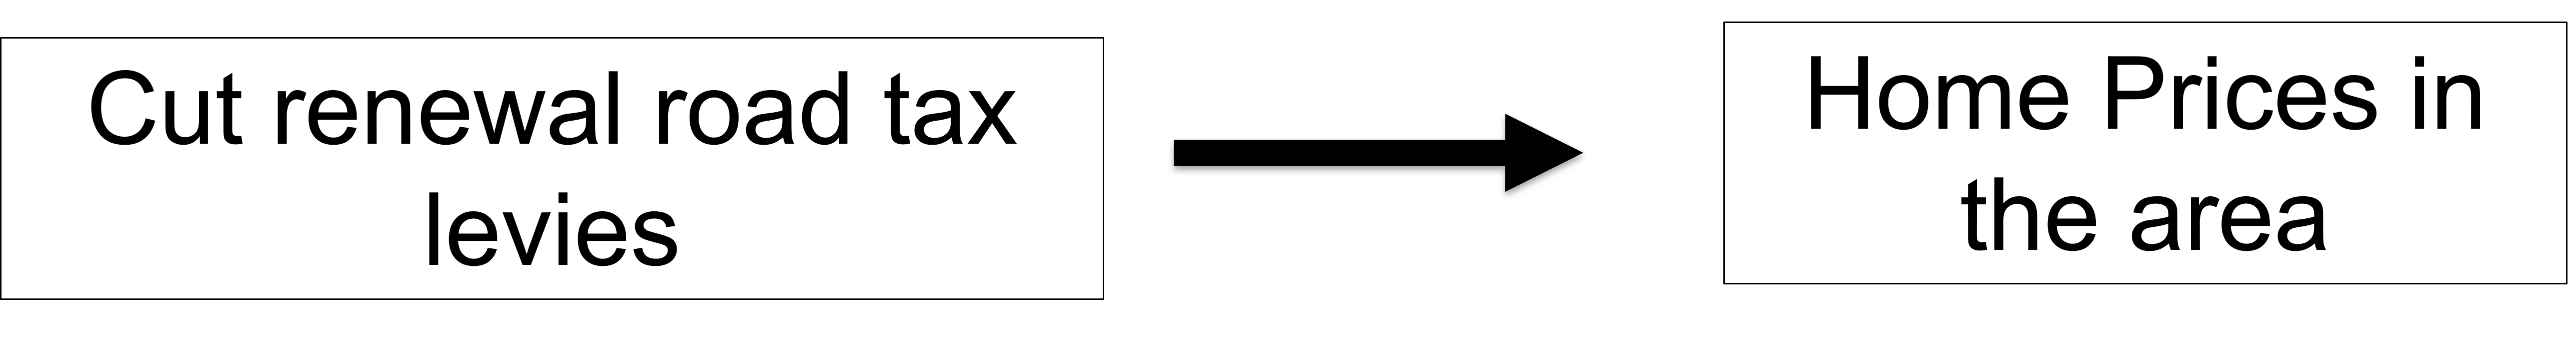
\includegraphics[width=0.8\textwidth]{images/research_question.png}
        \label{fig:research_question}
    \end{figure}
\end{frame}

\begin{frame}{Research Design - idea}    
    \begin{figure}[ht]
        \centering
        \begin{subfigure}{0.49\textwidth}
            \centering
            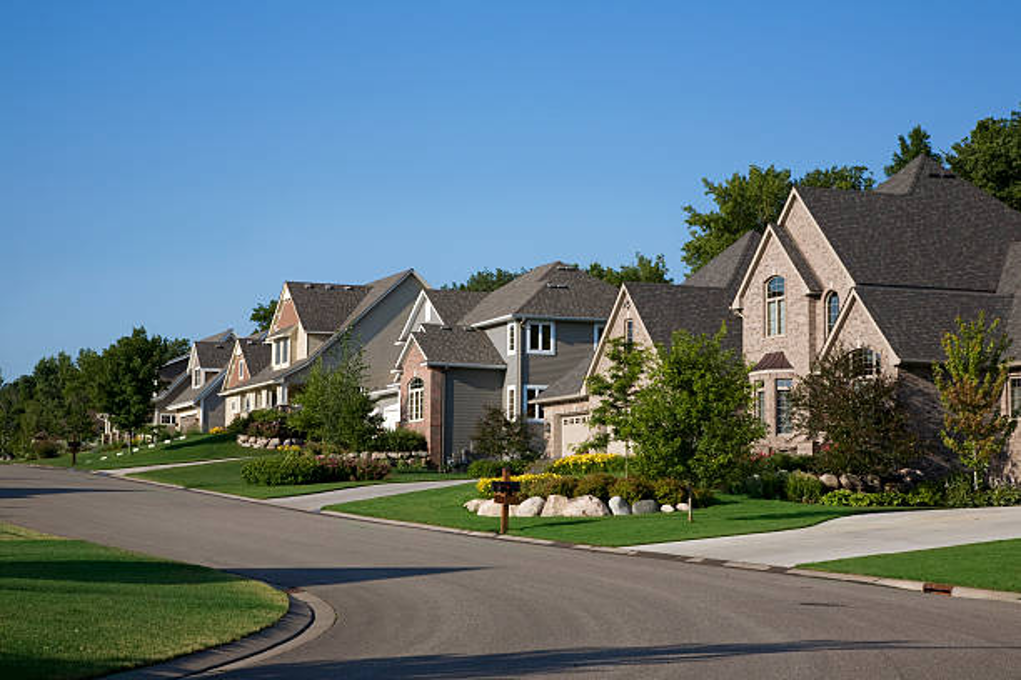
\includegraphics[width=\textwidth]{images/houses_good_roads.png}
            \caption{Houses with good roads}
            \label{fig:good_roads}
        \end{subfigure}
        \hfill
        \begin{subfigure}{0.49\textwidth}
            \centering
            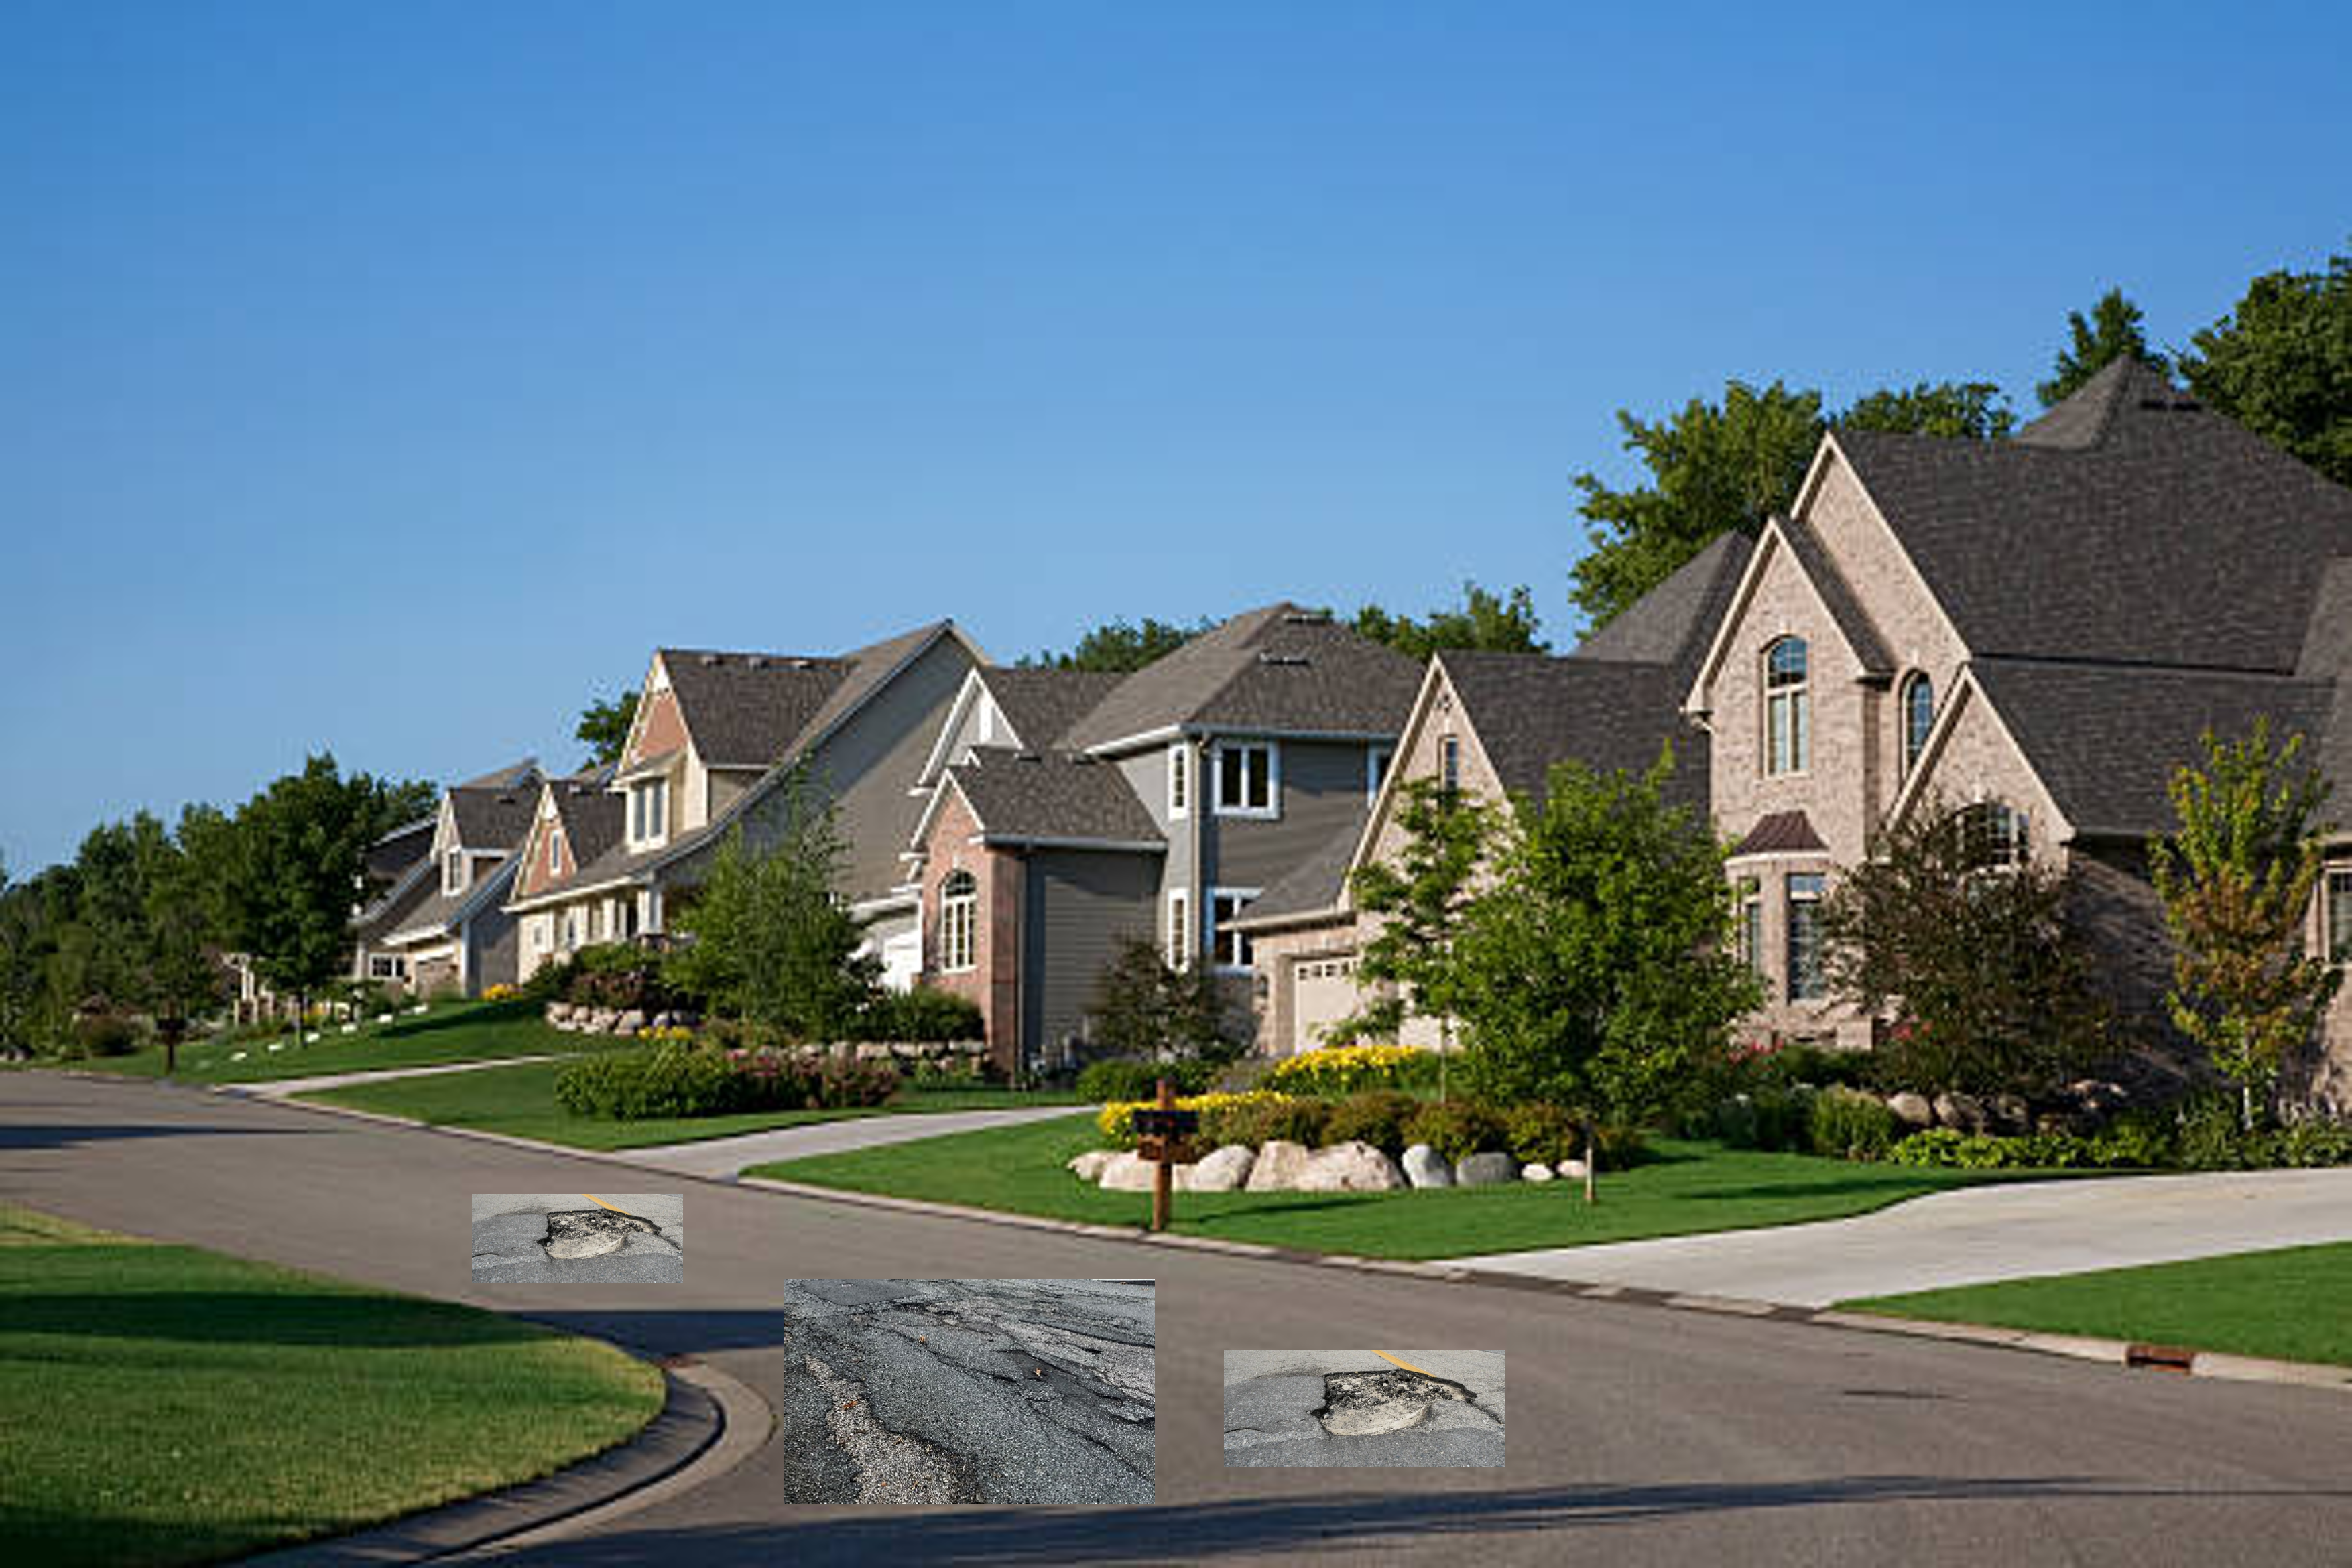
\includegraphics[width=\textwidth]{images/houses_bad_roads.png}
            \caption{Houses with bad roads}
            \label{fig:bad_roads}
        \end{subfigure}
        \caption{Comparing similar neighborhoods and only accounting for differences in roads}
        \label{fig:road_comparison}
    \end{figure}
\end{frame}

\begin{frame}{Running variable: \% votes against the renewal tax levy}
    \begin{itemize}
        \item Before a ``renewal tax levy'' can be renewed, it must be approved by the residents. So, elections are held every 5 years i.e. residents vote on whether they would like to be taxed or not
        \item We use the \textbf{percent of votes against} the renewal tax levy as the running variable
        \item If the percent of votes against the renewal tax levy is less than 50\%, the levy is renewed and it is part of our control group ($F_{it} = 0$). If it is more than 50\%, the levy is cut and it is part of our treatment group ($F_{it} = 1$).
    \end{itemize}
    \begin{flushright}
        \href{https://www.beavercreektwpohio.gov/319/Renewal-Road-Levy}{\beamergotobutton{Renewal proposal example}}
        \href{https://www.cleveland.com/community/2020/11/south-euclid-voters-approve-road-levy-renewal-mayfield-village-residents-pass-four-cleanup-issues.html}{\beamergotobutton{Renewal results example}}
    \end{flushright}
\end{frame}

\begin{frame}{Preview of Results}
    Median House Prices after 5 years: Control vs Treatment
    \begin{figure}[ht]
        \centering
        
\includegraphics[width=0.8\textwidth]{images/rd_plot_year_5_after_vote.png}
        \caption{5 years {\bf after} the vote}
        \label{fig:house_prices_before_after}
    \end{figure}
\end{frame}

\begin{frame}{Preview of Results}
    \begin{itemize}
        \item Loss of 11\% in maintenance funds from failing to renew a road tax levy
        \item Road quality rating drops by 0.44, which is about 15-40\% 
        \item \textbf{House prices}  declines of around \$15K (9\%) over a 10-year period
        \item \textbf{Urban vs. rural:} More consistent decline in urban areas compared to rural areas
        \item Higher-income neighborhoods experience larger absolute declines
        \item \textbf{Trade-off:} Tax savings for households today may not offset property value losses in the future
    \end{itemize}
\end{frame}

\begin{frame}{Line of Reasoning}
    \begin{itemize}
        \item Renewal tax levy failures reduce road maintenance funding
        \item Loss of maintenance funds contributes to poor road quality
        \item Road quality declines soon after a tax renewal levy fails
    \end{itemize}
    \begin{figure}[ht]
        \centering
        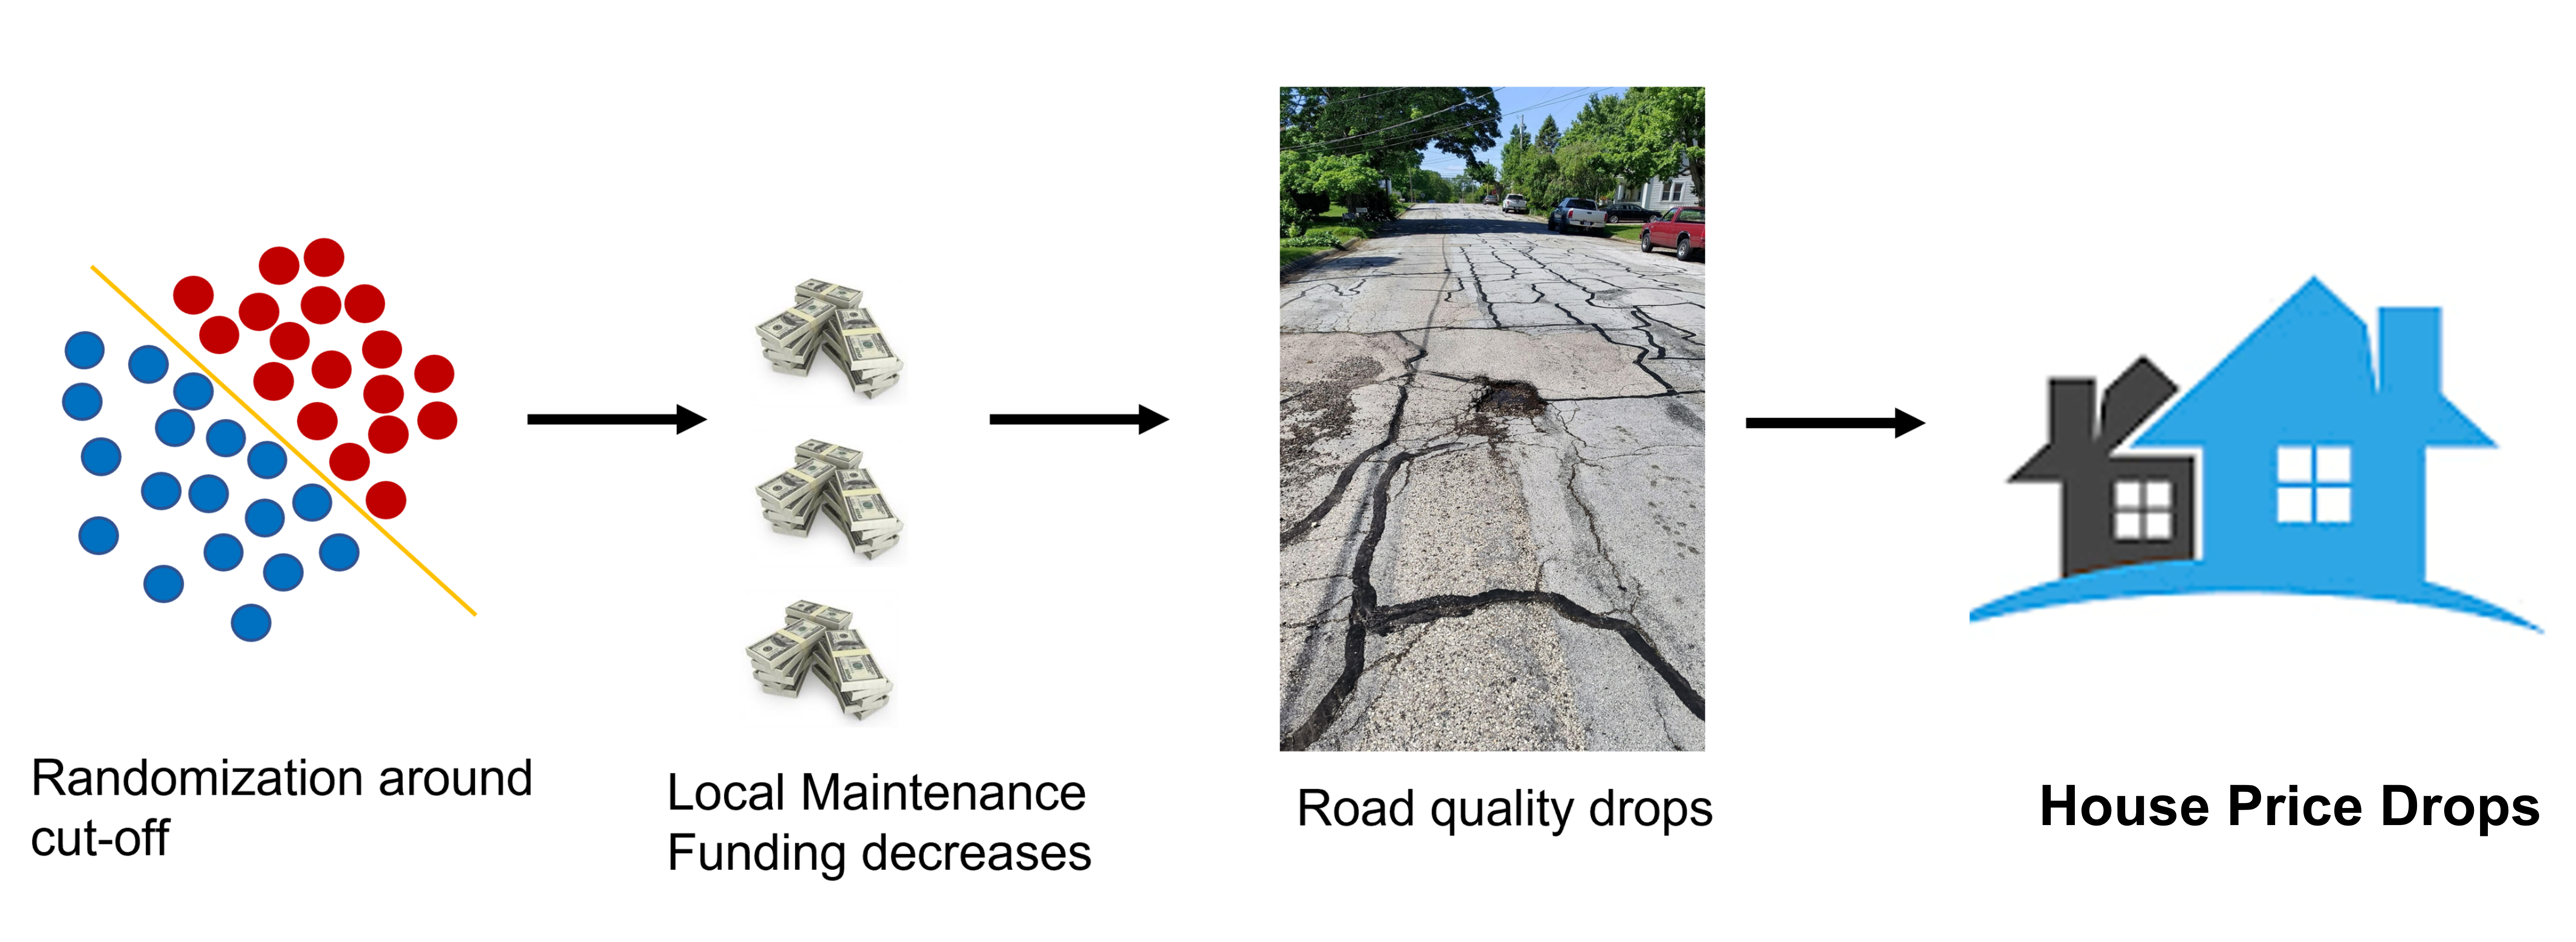
\includegraphics[width=0.8\textwidth]{images/approach.png}
        \caption{High-level Overview}
        \label{fig:approach}
    \end{figure}
\end{frame}

\begin{frame}{Contribution}
    \begin{itemize}
        \item We provide novel measures of impact of infrastructure maintenance by constructing a \textbf{unique dataset} linking:
            \begin{itemize}
                \item Local referendum results
                \item Financial audit reports
                \item Satellite and Streetview road images
                \item Housing transactions
            \end{itemize}
        \item Focus on \textbf{long-term impacts} of cutting a specific-purpose tax
        \item Emphasize the \textbf{role of infrastructure maintenance} in a developed economy
    \end{itemize}
\end{frame}

%-------------------------------------------------------
% Section 2: Background & Literature Review
%-------------------------------------------------------
\section{Background \& Lit Review}

\begin{frame}[label=who_funds_roads]{Background}
    Who funds the roads in Ohio?
    \begin{itemize}
        \item {\bf Federal Government: } New project grants
        \item {\bf State Government: } Inter-state highways and arterial roads
        \item {\bf Local Governments: } Local roads 
    \end{itemize}

    \begin{flushright}
        \hyperlink{odot_who_does_what}{\beamergotobutton{ODOT Source}}
    \end{flushright}

    How are roads funded in Ohio?
    \begin{itemize}
        \item {\bf Gas taxes:} Federal (\$0.18 per gallon) and state (\$0.38 per gallon)
        \item {\bf User taxes:} Licensing, registration fees, tolls etc.
        \item {\bf Property taxes:} unvoted (10-mill rule) and \textcolor{red}{\bf voted} (road tax levies - must be approved by residents) 
    \end{itemize}
\end{frame}

\begin{frame}{Local Taxation in Ohio}
    \begin{itemize}
        \item 88 counties: Divided in townships, villages and cities
        \item Property tax collected by County Tax Assessor, distributed by county to local governments
        \item ORC has a 10-mill limit on unvoted levies. Additional property tax must be voted upon and approved by the residents
        \item Property tax is on assessed value, 35\% of appraised value of the property
        \item Example of a typical levy:

        2-mill, 5-year renewal road tax levy in Adams Township in 1995

    \end{itemize}
\end{frame}

\begin{frame}{Literature Review}
    % \begin{itemize}[<+->] 
    \begin{itemize}
        \item \textbf{Regression Discontinuity (RD) on new roads}: Asher and Novosad (2020) study the impact of new local roads on economic outcomes in India 
        \item \textbf{Local elections and referendums:} 
        \begin{itemize}
            \item Cellini, Ferreira and Rothstein (2010), Biasi, Lafortune and Schönholzer (2025)
        \end{itemize}
        \item \textbf{Method: Dynamic RD estimator}
        \begin{itemize}
            \item Cellini, Ferreira, and Rothstein (2010)
        \end{itemize}
        \item {\bf Oates' Decentralization Theorem (1972)} suggests that local governments are better suited to provide local public goods, such as road maintenance, than higher levels of government.
    \end{itemize}
    % \vspace{0.5cm}
    % \begin{flushright}
    %     \textbf{\hyperlink{references}{See References in Appendix}}
    % \end{flushright}
\end{frame}


%-------------------------------------------------------
% Section 3: Data & Methodology
%-------------------------------------------------------
\section{Data, Spending \& House prices}

\begin{frame}{Data Sources}
    \begin{itemize}
        \item \textbf{Local Election Results:} Ohio Secretary of State
        \vskip 0.5cm
        \item \textbf{Housing Prices:} CoreLogic
        \vskip 0.5cm
        \item \textbf{Spending Data:} Audited Financial Reports from Ohio Auditor of State 
        \vskip 0.5cm
        \item \textbf{Road Images:} \textit{Brewer et al. (2021) Satellite images dataset}, Google Earth, Google Maps Streetview API, Kaya and Çodur (2022, 2024) street images
    \end{itemize}
\end{frame}


\begin{frame}{Spending Measures}
    \begin{itemize}
        \item \textbf{Metric 1:} Estimated loss in road maintenance funds
        \vskip 0.2cm
        
         Loss $=$ Avg Millage Rate $\times$ 0.35 $\times$ Avg. Appraised Value $\times$ \# Households

         \vskip 0.5cm
        \item \textbf{Metric 2:} Spending regression on Road Tax cuts
        $$ Spending = f(Tax \ Cuts)$$
    \end{itemize}
\end{frame}

\begin{frame}{Spending measures: Metric 1 results}
    \begin{table}[ht]
        \centering
        \caption{Spending impact of failing to renew a Road Tax Levy}
        \label{tab:levy_stats}
        \begin{threeparttable}
        \begin{tabular}{p{4.5cm}ccc}
        \hline\hline
        & \textbf{Aggregate} & \textbf{Renewed} & \textbf{Cut} \\
        \hline
        \textbf{Panel A: road tax per household} \\
        Mean & 76 & 75 & 79 \\
           & (55) & (53) & (62) \\
        \hline
        \textbf{Panel B: road tax per city} \\
        Mean & 167,011 & 167,648 & 163,547 \\
           & (340,268) & (340,628) & (338,671) \\
        \hline\hline
        \end{tabular}
        \begin{tablenotes}[flushleft]
          \footnotesize
          \item \textit{Notes:} 
          This table presents descriptive statistics for two measures of the money collected via road tax levies. 
          \textbf{Panel A} reports the mean and standard deviation (SD) of the road tax per household per year. 
          \textbf{Panel B} reports the mean and SD of the total road tax collected per city. 
          “Aggregate” denotes the full sample, while “Renewed” and “Cut” refer to levies that were renewed and failed to renew respectively.
        %   All monetary values are in constant 2010 U.S. dollars and rounded to the nearest integer.
        \end{tablenotes}
        \end{threeparttable}
    \end{table}    
\end{frame}

\begin{frame}{Spending measures: Metric 2 work-in-progress}
    \begin{itemize}
        \item We scraped Ohio Auditor of State website to collect all available financial reports for townships, cities and villages. This gives us over 10,000 reports.
        \item Reports contain taxes collected and expenditures incurred by the local government, for various purposes. 
        \item  We will check the immediate or eventual changes in funding after a tax cut.
    \end{itemize}
\end{frame}

\begin{frame}{Identification Strategy}
    We use a dynamic \textbf{Dynamic Regression Discontinuity (RD)} design and operationalize CFR (2010)-inspired estimator using the following equation-
        \begin{equation}
            Y_{i,t+\tau} = \alpha_\tau + \kappa_t + F_{it} \theta_{\tau}^{ITT} + P_g (v_{it}, \gamma_\tau) + Z_{it} \beta_\tau + \epsilon_{i,t + \tau}
            \label{eq:itt_estimator}
        \end{equation}
        \begin{itemize}
            \item[] \scriptsize $Y_{i,t+\tau}$: Outcome variable for city $i$ at year $t + \tau$.
            \item[] \scriptsize $F_{it}$: Indicator variable representing the failure of a city, village, or township to renew its road maintenance tax levy.
            \item[] \scriptsize $\theta_{\tau}^{ITT}$: Causal effect of failing to renew the road tax levy on the outcome.
            \item[] \scriptsize $P_g (v_{it}, \gamma_\tau)$: Polynomial function of the running variable $v_{it}$, which is the percent of votes against the renewal tax levy.
            \item[] \scriptsize $\alpha_\tau$: Timing-specific fixed effects.
            \item[] \scriptsize $\kappa_t$: Year-specific fixed effects.
            \item[] \scriptsize $Z_{it}$: Vector of control variables, including city-level demographics, economic conditions, and other relevant covariates.
            \item[] \scriptsize $\epsilon_{i,t + \tau}$: Error term capturing unobserved factors.
        \end{itemize}
\end{frame}

\begin{frame}{Results: Effect of road tax cuts on House prices}
    \begin{table}[ht]
    \centering
    \caption{\scriptsize Effect on median house prices of failing to renew a road tax levy}
    \label{tab:median_sale_amount}
    \resizebox{\textwidth}{!}{%
    \begin{tabular}{p{2.5cm}ccccccc}
    \hline
    \scriptsize Year relative to vote & \scriptsize $t + 4$ & \scriptsize $t + 5$ & \scriptsize $t + 6$ & \scriptsize $t + 7$ & \scriptsize $t + 8$ & \scriptsize $t + 9$ & \scriptsize $t + 10$ \\
    \hline
    \scriptsize Treatment effect & \scriptsize -21,638 & \scriptsize -22,271 & \scriptsize -17,336 & \scriptsize -15,975 & \scriptsize -21,993 & \scriptsize -19,857 & \scriptsize -16,090 \\
    \scriptsize Standard error   & \scriptsize (7,731) & \scriptsize (8,864) & \scriptsize (8,331) & \scriptsize (7,248) & \scriptsize (9,079) & \scriptsize (7,751) & \scriptsize (9,027) \\
    \scriptsize Effective bandwidth ($h$) & \scriptsize 8.540 & \scriptsize 10.796 & \scriptsize 9.840 & \scriptsize 13.158 & \scriptsize 8.246 & \scriptsize 7.285 & \scriptsize 6.241 \\
    \scriptsize Bias bandwidth ($b$) & \scriptsize 16.379 & \scriptsize 19.879 & \scriptsize 17.397 & \scriptsize 23.413 & \scriptsize 15.255 & \scriptsize 14.091 & \scriptsize 16.266 \\
    \scriptsize Effective Observations & \scriptsize 688 & \scriptsize 883 & \scriptsize 769 & \scriptsize 1,061 & \scriptsize 591 & \scriptsize 505 & \scriptsize 402 \\
    \scriptsize Total Observations & \scriptsize 2,614 & \scriptsize 2,531 & \scriptsize 2,438 & \scriptsize 2,324 & \scriptsize 2,199 & \scriptsize 2,115 & \scriptsize 2,017 \\
    \hline
    \end{tabular}%
    }
    \vspace{-0.2cm}
    \begin{tablenotes}
    \scriptsize
    \item \textit{Notes:} Outcome is median house price in constant 2010 U.S. dollars. Unit of observation is the city-year. Treatment effects for years prior to $t + 4$ are statistically insignificant at the 5\% level. The regressions include covariates related to the demographics and socioeconomic factors of the cities, drawn from covariates table (see Appendix) .
    \end{tablenotes}
    \end{table}
    {\bf \$15K or about 9\% over 10 years}
\end{frame}


\begin{frame}{Results: Effect of road tax cuts on House prices}
    \begin{figure}[ht]
        \centering
        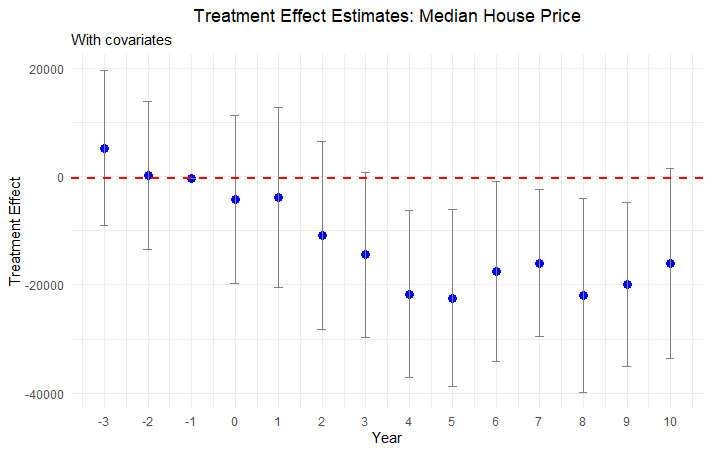
\includegraphics[width=0.85\textwidth]{images/tes_gs_reg.png}
        \caption{Year-by-year estimate of the effect of failing to renew a road tax levy on median house prices}
        \label{fig:tes_gs_re}
    \end{figure}    
\end{frame}

\begin{frame}{Results: Urban vs. Rural}
    \begin{figure}[ht]
        \centering
        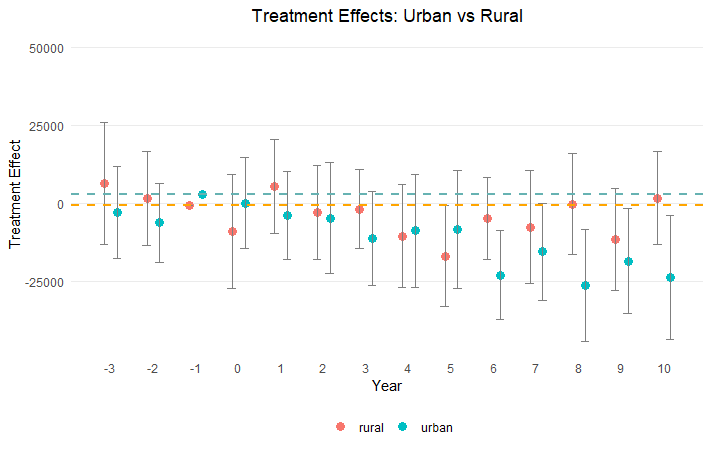
\includegraphics[width=0.85\textwidth]{images/tes_covs_ua_reg.png}
        \caption{Urban vs Rural}
        \label{fig:tes_covs_ua_reg}
    \end{figure}    
    {7.6\% of the home price over 10 years}
\end{frame}

\begin{frame}{Results: Expenses vs Cheaper Houses} 
    \begin{figure}[ht]
        \centering
        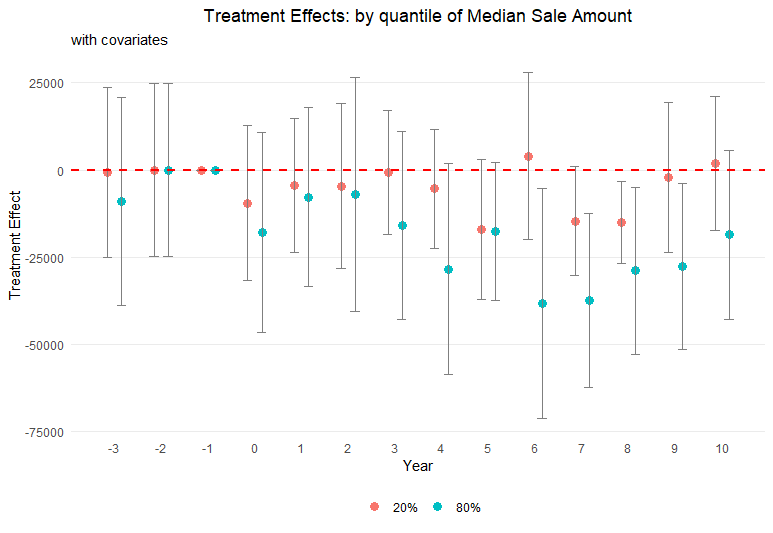
\includegraphics[width=0.85\textwidth]{images/tes_qte_re.png}
        \caption{Quantile Treatment Effects}
        \label{fig:tes_qte_re}
    \end{figure}    
\end{frame}


%-------------------------------------------------------
% Section 4: Road Quality
%-------------------------------------------------------
\section{Road Quality}

\begin{frame}{Road Quality Measures}
    \begin{itemize}
        \item \textbf{Satellite-based approach:}
            \begin{itemize}
                \item Using labeled data from Brewer et al. (2021)
                \item Fine-tune a Vision Transformer model for road quality classification
                \item Collect Ohio images from Google Earth
                \item Compare \textbf{pre- vs. post-election} images in the same localities
            \end{itemize}
        \vskip 0.5cm
        \item \textbf{Street-view images approach:}
            \begin{itemize}
                \item Use Kaya and Çodur (2024) labeled dataset
                \item Leverage Google Streetview API for collecting Ohio images
                \item Compare \textbf{pre- vs. post-election} images in the same localities
            \end{itemize}
    \end{itemize}
    We will show you first our method and results from our work on satellite images.
\end{frame}

\begin{frame}{Road Quality, Method 1: Satellite images}
    \begin{itemize}
        \item Brewer et al (2021) provides 53,000 labeled Satellite Images of roads in U.S.
        \item They use Google’s Inception V3 ML model to classify road quality into 3 categories:
            \begin{itemize}
                \item 0 for "Low" quality road
                \item 1 for "Medium" quality road
                \item 2 for "High" quality road
            \end{itemize}
        \item We use their images to fine-tune GPT-4O model by Open AI. This multi-modal model has Vision capabilities, meaning it can “see” things and infer
    \end{itemize}
\end{frame}

\begin{frame}{Road Quality: Brewer's Training Data}
    \begin{figure}[ht]
        \centering
        \begin{subfigure}{0.32\textwidth}
            \centering
            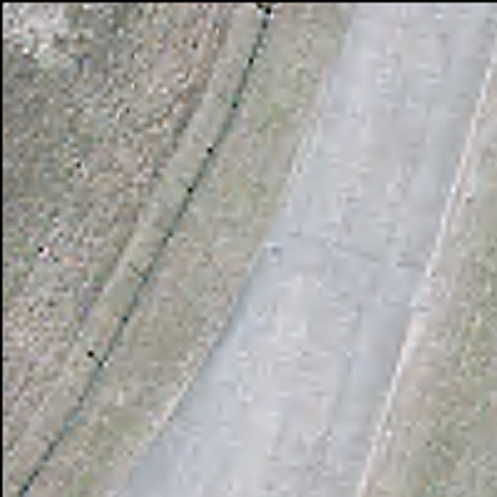
\includegraphics[width=\textwidth]{images/brewer_road_low.png}
            \caption{"Low" quality road}
            \label{fig:low_quality}
        \end{subfigure}
        \hfill
        \begin{subfigure}{0.32\textwidth}
            \centering
            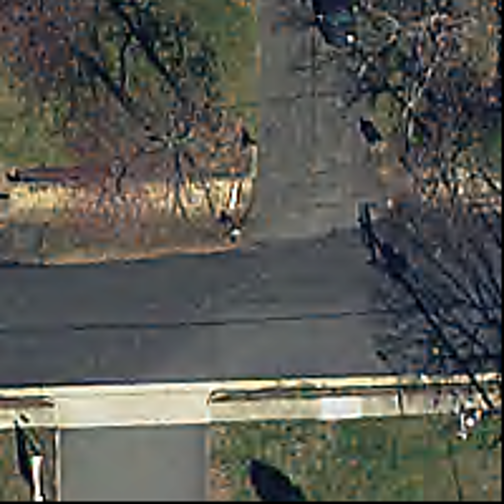
\includegraphics[width=\textwidth]{images/brewer_road_medium.png}
            \caption{"Med" quality road}
            \label{fig:medium_quality}
        \end{subfigure}
        \hfill
        \begin{subfigure}{0.32\textwidth}
            \centering
            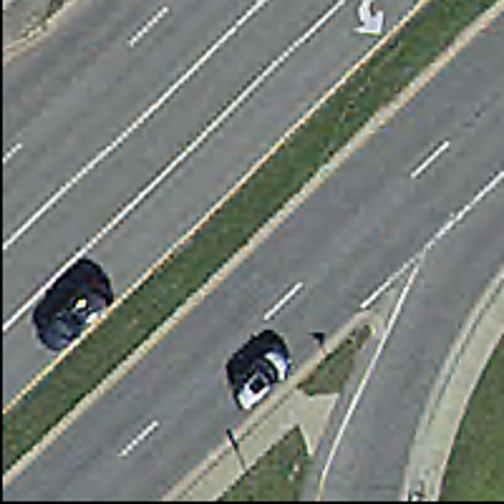
\includegraphics[width=\textwidth]{images/brewer_road_high.png}
            \caption{"High" qualiy road}
            \label{fig:high_quality}
        \end{subfigure}
        \caption{Examples: Satellite images of roads in Brewer et al. (2021)}
        \label{fig:road_quality_egs}
    \end{figure}
\end{frame}

\begin{frame}{Road Quality: fine-tuning workflow}
    \begin{figure}[ht]
        \centering
        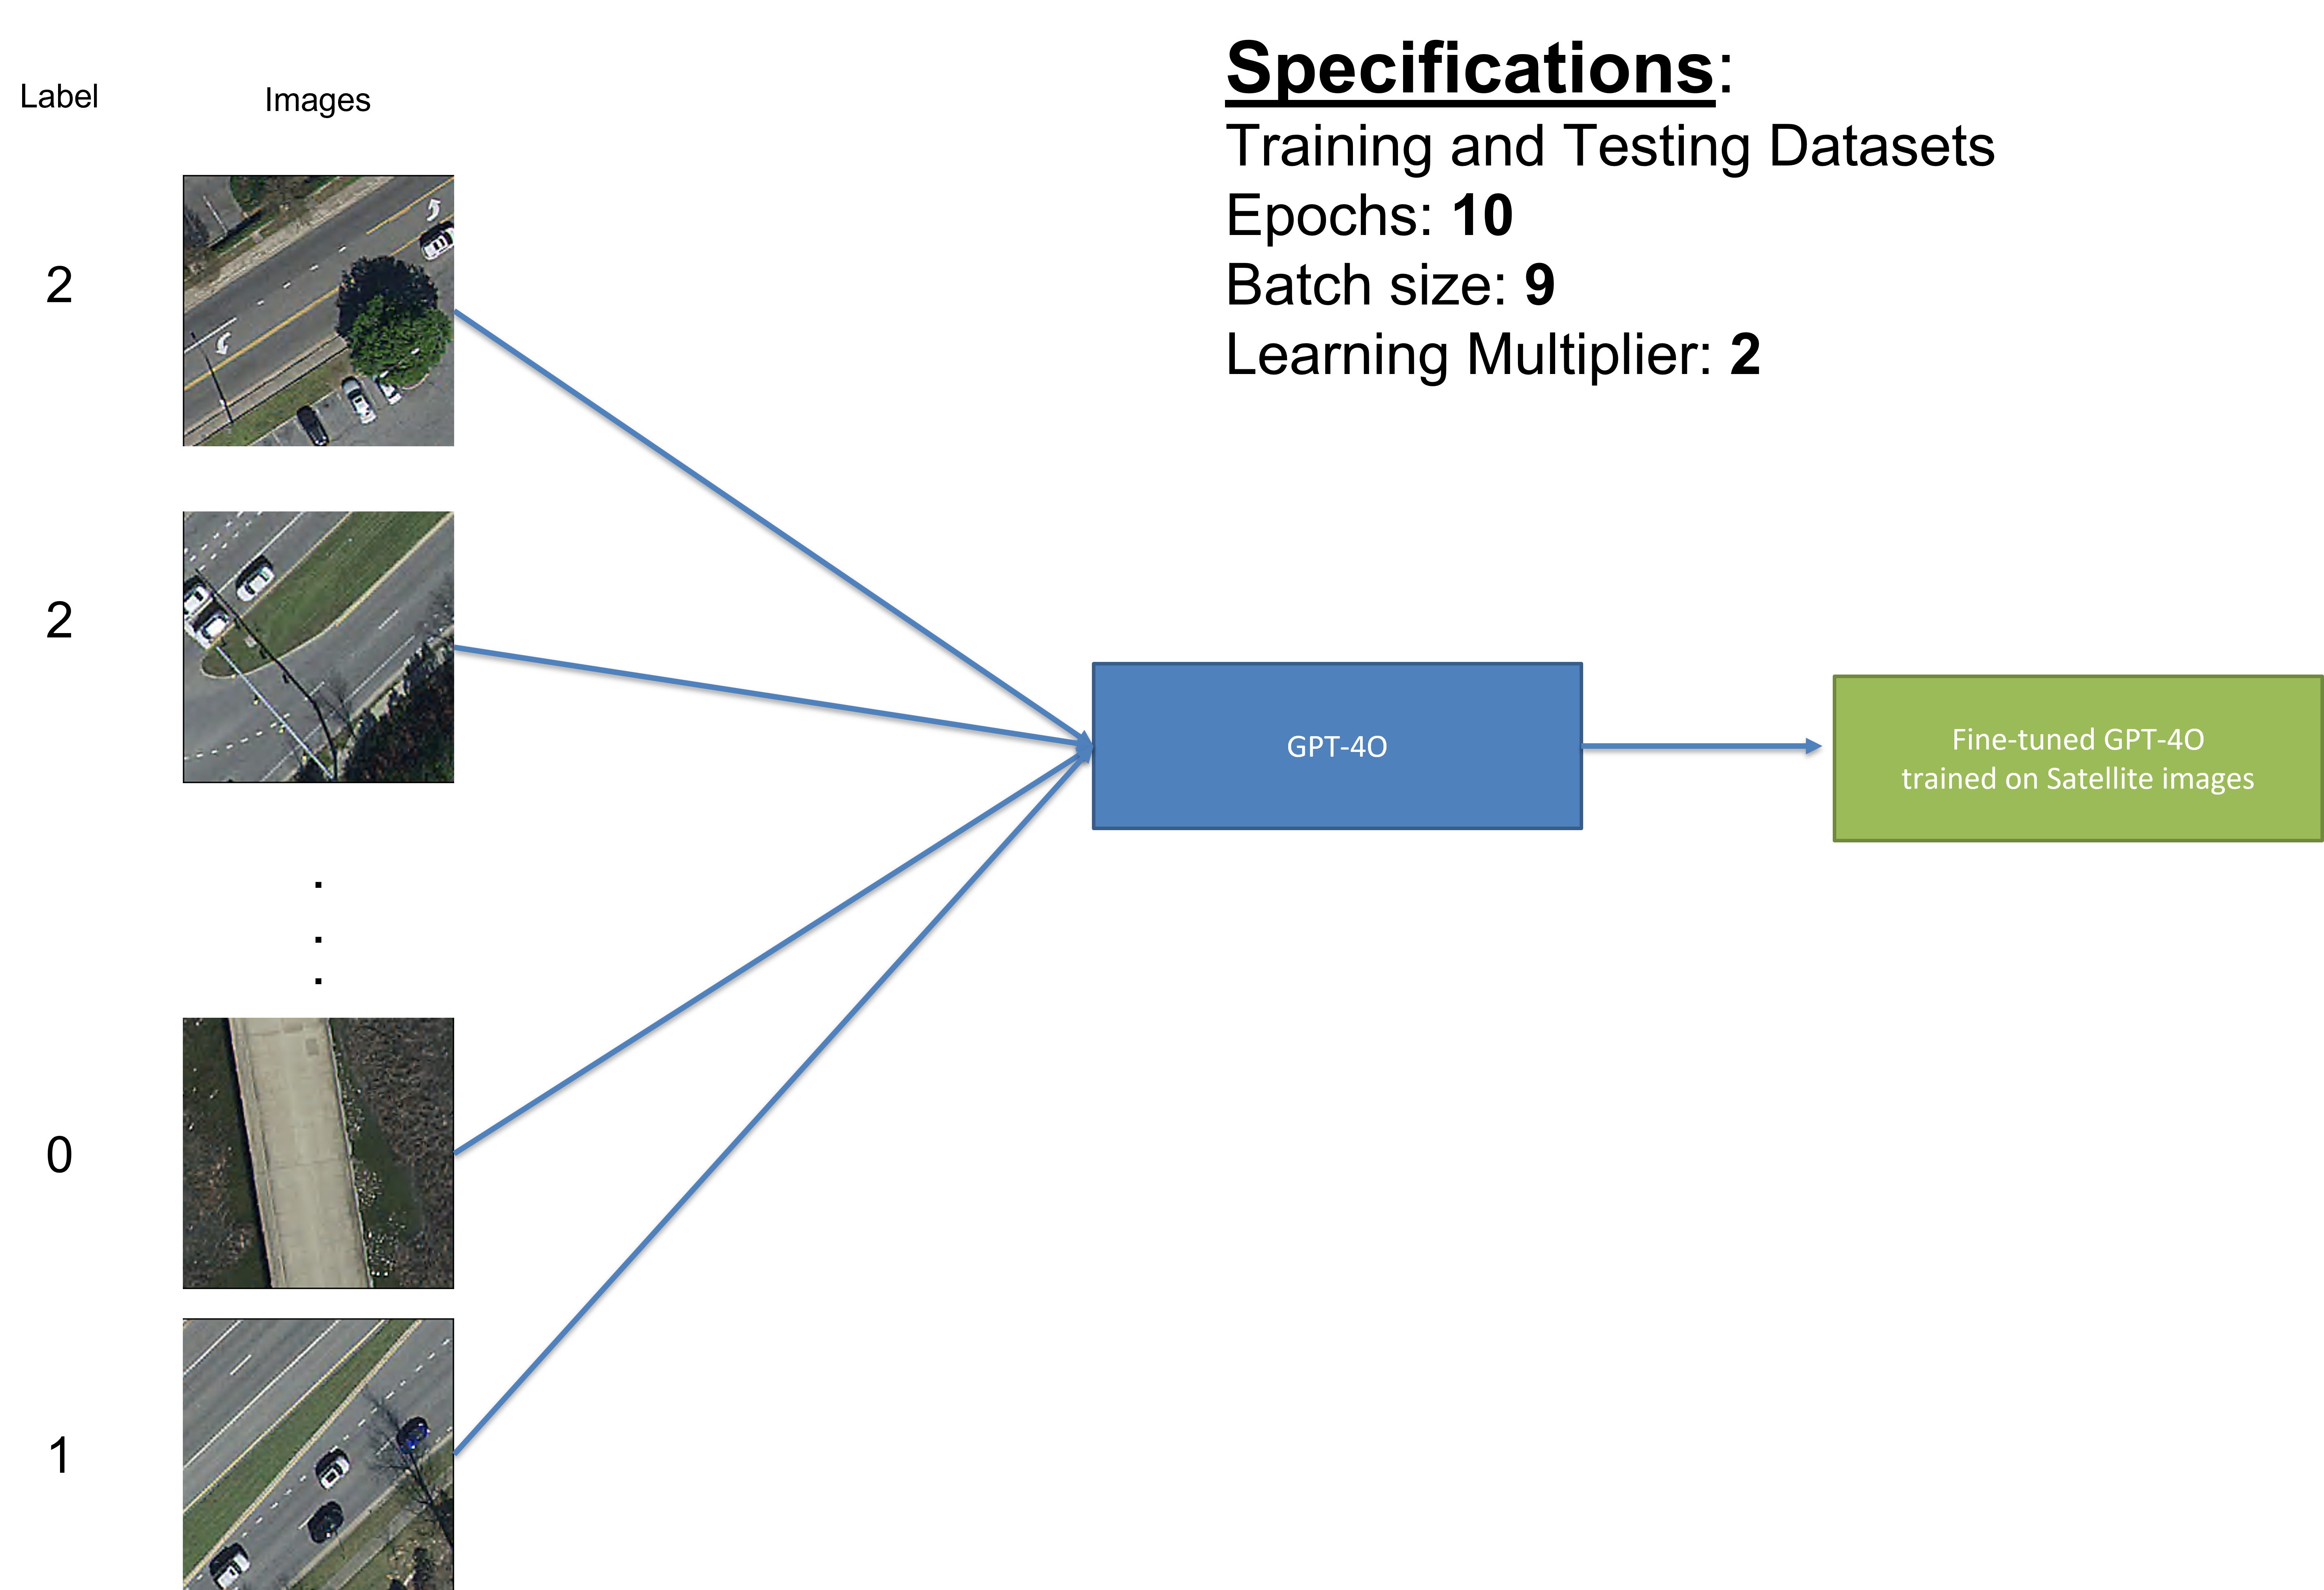
\includegraphics[width=0.9\textwidth]{images/fine_tuning_workflow.png}
        \caption{Fine-tuning workflow for road quality classification}        
        \label{fig:road_quality_workflow}
    \end{figure}
\end{frame}

\begin{frame}{Road Quality: Ohio satellite images}
    We use fine-tuned GPT 4O to predict the quality of Ohio Satellite Images collected from Google Earth.
    \begin{figure}[ht]
        \centering
        \begin{subfigure}{0.49\textwidth}
            \centering
            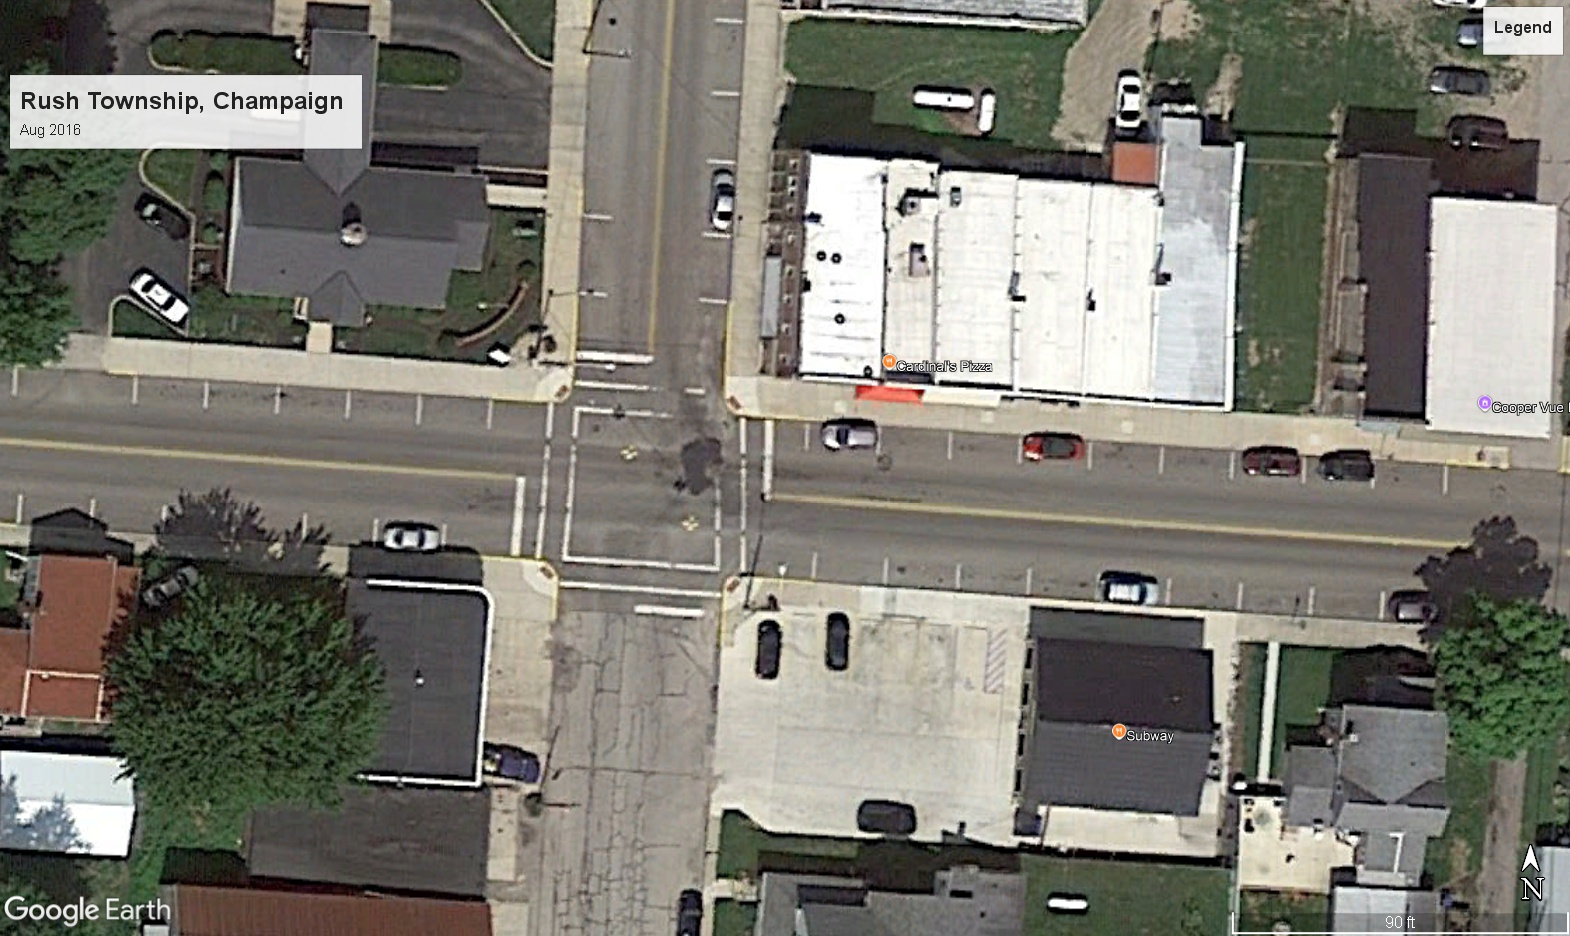
\includegraphics[width=\textwidth]{images/rush_twp_champaign_aug16.jpg}
            \caption{Road predicted as "Low" (0) quality}
            \label{fig:rush16}
        \end{subfigure}
        \hfill
        \begin{subfigure}{0.49\textwidth}
            \centering
            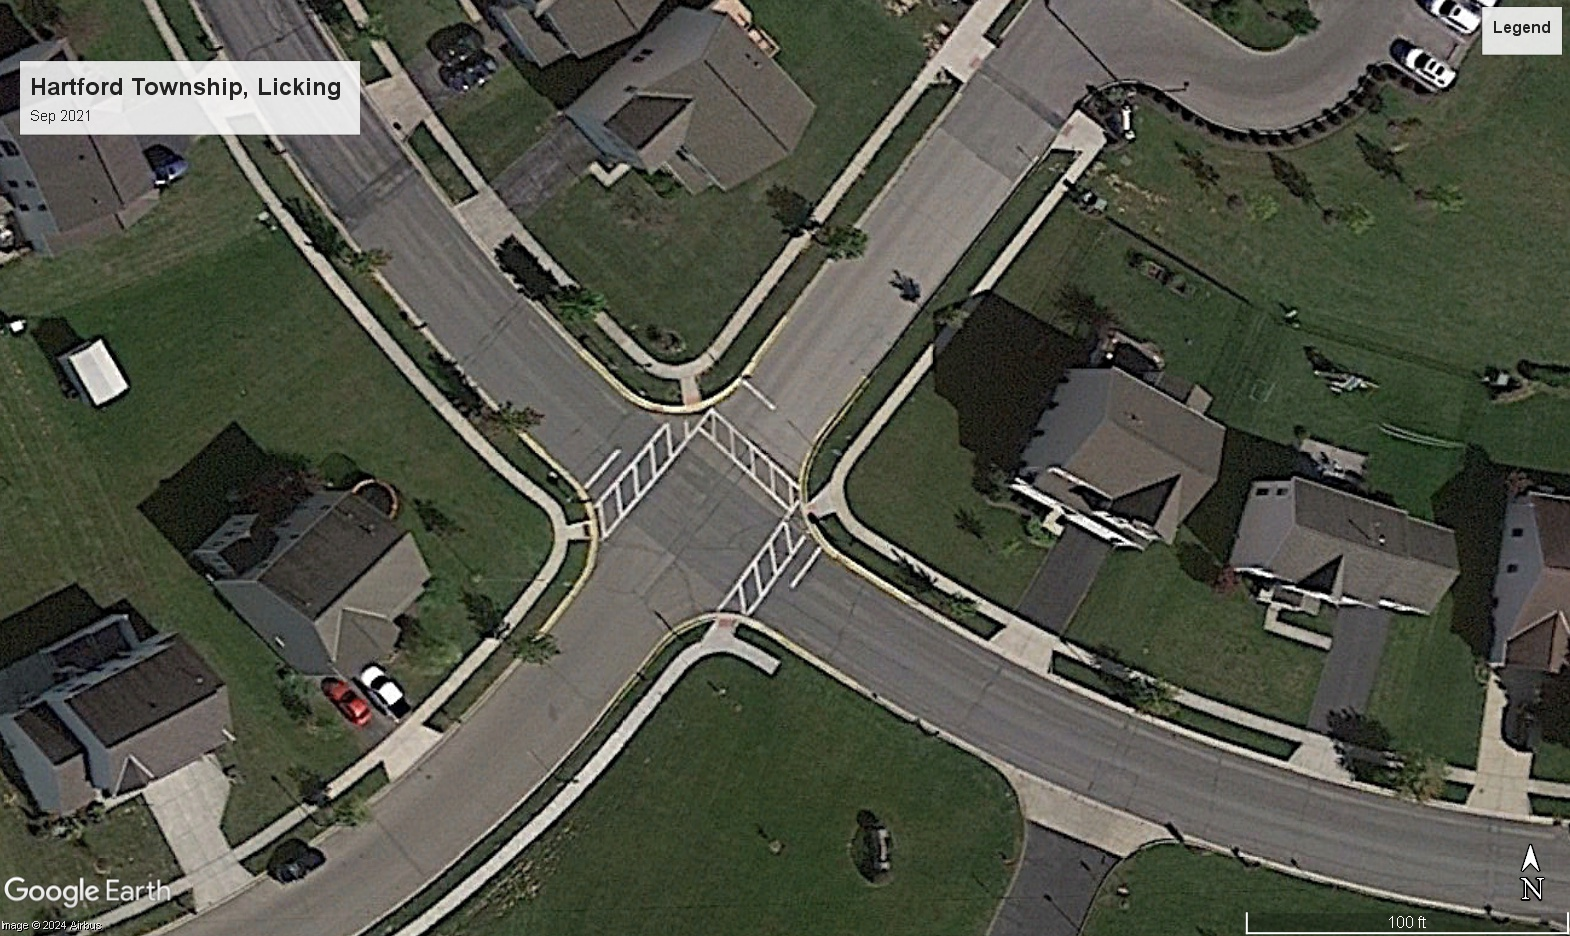
\includegraphics[width=\textwidth]{images/hartford_twp_licking_sep21.jpg}
            \caption{Road predicted as "High" (2) quality}
            \label{fig:hartford21}
        \end{subfigure}
        % \caption{Overall caption for the two images}
        \label{fig:ohio_satellite_images}
    \end{figure}

    Fine-tuned model results: Brewer’s metric of 70\%
\end{frame}

\begin{frame}{Road Quality: Ohio satellite images}
    We are interested in the {\bf change} in road quality before and after each election.
    \begin{figure}[ht]
        \centering
        \begin{subfigure}{0.49\textwidth}
            \centering
            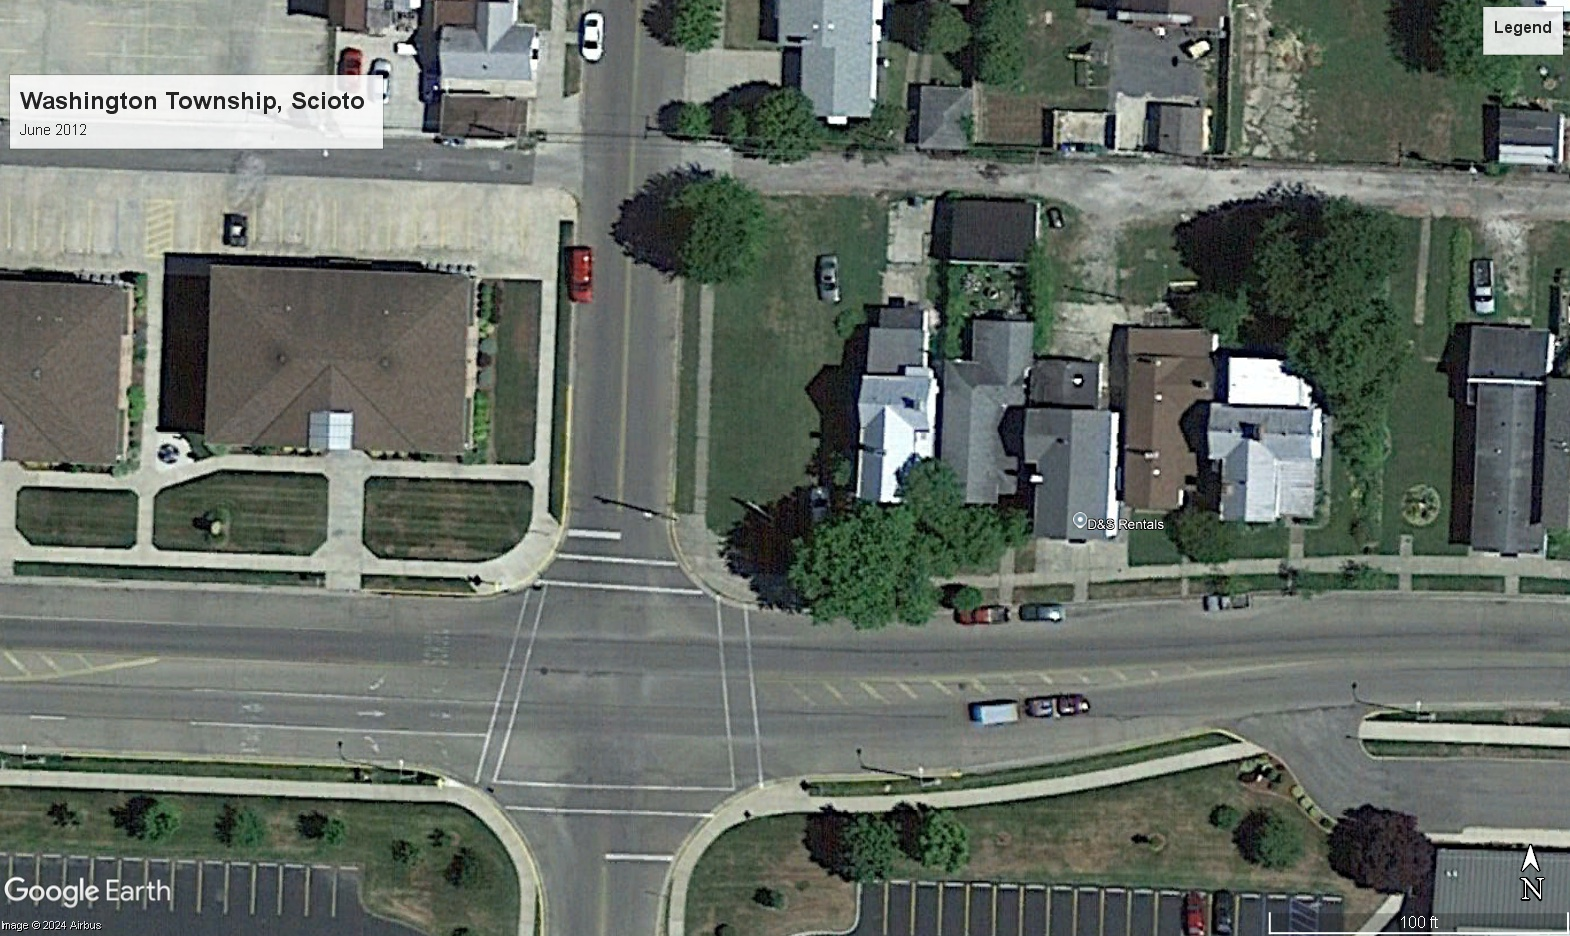
\includegraphics[width=\textwidth]{images/washington_twp_scioto_jun2012.jpg}
            \caption{Road predicted as "High" (2)}
            \label{fig:pred_2}
        \end{subfigure}
        \hfill
        \begin{subfigure}{0.49\textwidth}
            \centering
            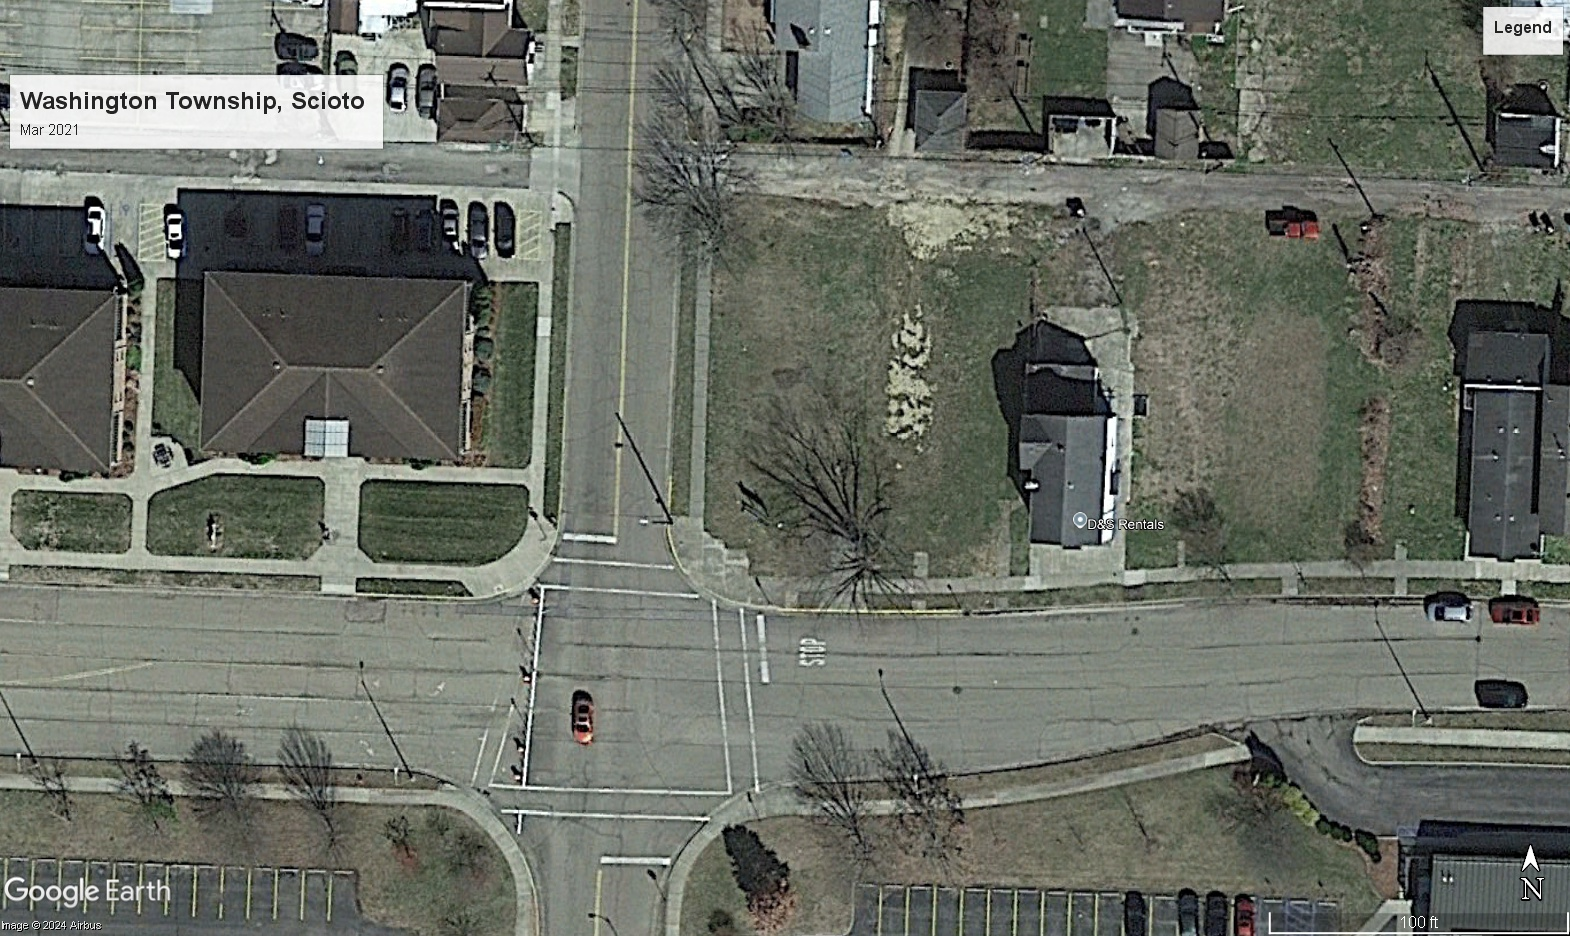
\includegraphics[width=\textwidth]{images/washington_twp_scioto_mar21.jpg}
            \caption{Road predicted as "Medium" (1)}
            \label{fig:pred_1}
        \end{subfigure}
        \caption{Washington Township, Scioto County, Ohio - 2012 vs. 2021}
        \label{fig:washington_pred}
    \end{figure}
\end{frame}

\begin{frame}{Results: Road quality decline}
    \begin{table}[ht]
        \centering
        \caption{\scriptsize Effect of Referendum Outcome on Road Quality}
        \label{tab:roadquality_estimates}
        \resizebox{\textwidth}{!}{%
        \begin{threeparttable}
        \begin{tabular}{lcc}
        \hline\hline
         & \textbf{\scriptsize Cut Levies} & \textbf{\scriptsize Maintained Levies} \\
        \hline
        \\[-0.3cm]
        \scriptsize Change in Road Quality after a Referendum 
         & \scriptsize -0.444\textsuperscript{**} & \scriptsize 0.067 \\[0.2cm]
         & \scriptsize (0.210) & \scriptsize (0.340) \\  
        \hline
        \end{tabular}
        \begin{tablenotes}
        \scriptsize
        \item \textit{Notes:} Each column represents an estimate of change in road quality from OLS regression for the set of cities that cut and renew their road tax levies. Samples are the set of referendums within the mean effective RD bandwidth from Table \ref{tab:median_sale_amount}. “Cut Levies” refers to jurisdictions that failed to renew their road tax levies, while “Maintained Levies” refers to jurisdictions that renewed. Standard errors are shown in parentheses. 
        \item Significance levels: 
        \textsuperscript{*}p $<$ 0.10,  
        \textsuperscript{**}p $<$ 0.05, 
        \textsuperscript{***}p $<$ 0.01.
        \end{tablenotes}
        \end{threeparttable}%
        }
    \end{table}
    {\bf This corresponds to 15-40\% deterioration in road quality.}
\end{frame}

\begin{frame}{Road quality, Method 2: Streetview images}
    \begin{center}
        Kaya, Yasin (2024): Road damage labeled Streetview data from 6 different countries.
        \begin{figure}[ht]
            \centering
            \begin{subfigure}{0.49\textwidth}
                \centering
                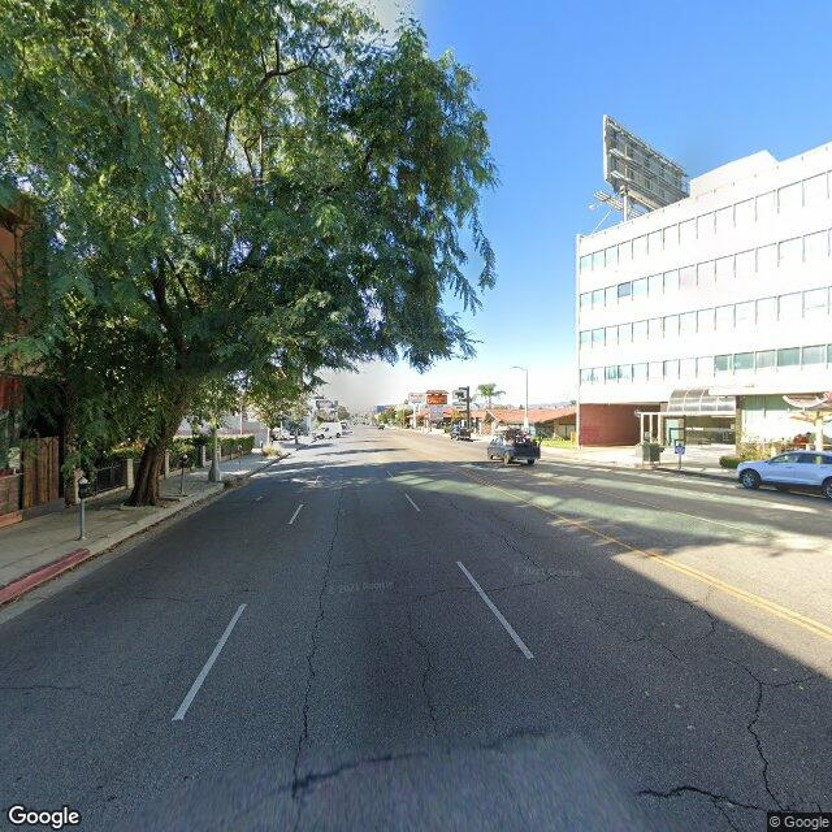
\includegraphics[width=\textwidth]{images/streetview_training_data_example.jpg}
                \caption{000122}
                \label{fig:streetview_image1}
            \end{subfigure}
            \hfill
            \begin{subfigure}{0.49\textwidth}
                \centering
                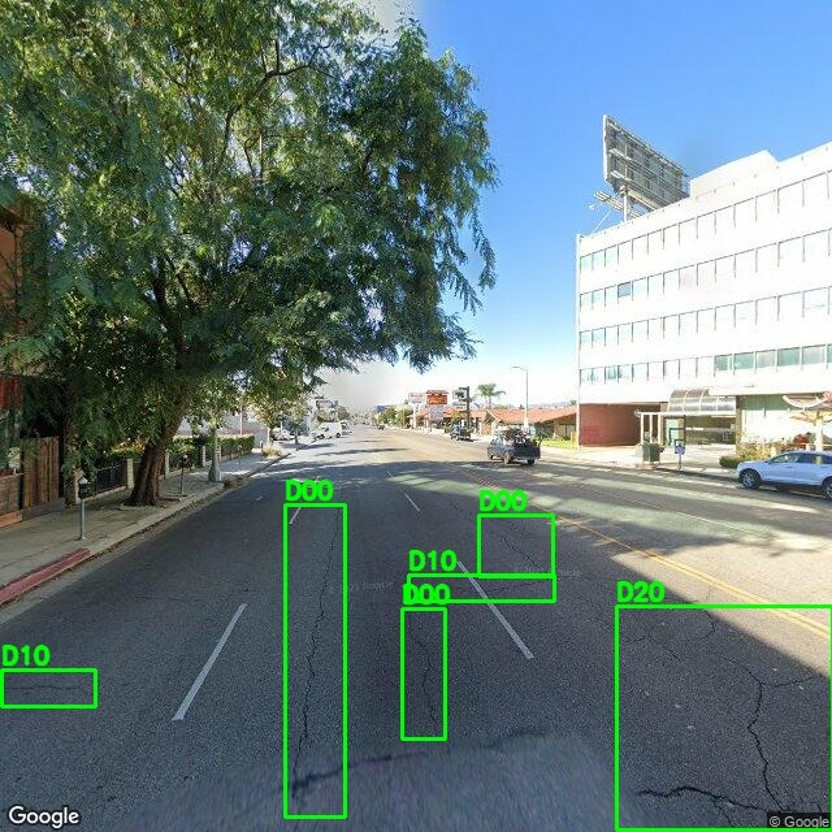
\includegraphics[width=\textwidth]{images/streetview_training_data_example_labeled.jpg}
                \caption{000122 - labeled}
                \label{fig:streetview_image2}
            \end{subfigure}
            % \caption{Overall caption for the two images}
            % \label{fig:side_by_side_images}
        \end{figure}
    \end{center}
\end{frame}

\begin{frame}{Road quality, Method 2: Streetview images}
    \begin{center}
        Using Google Streetview API, we collect Streetview images before and after an election in a subdivision.
        \begin{figure}[ht]
            \centering
            \begin{subfigure}{0.49\textwidth}
                \centering
                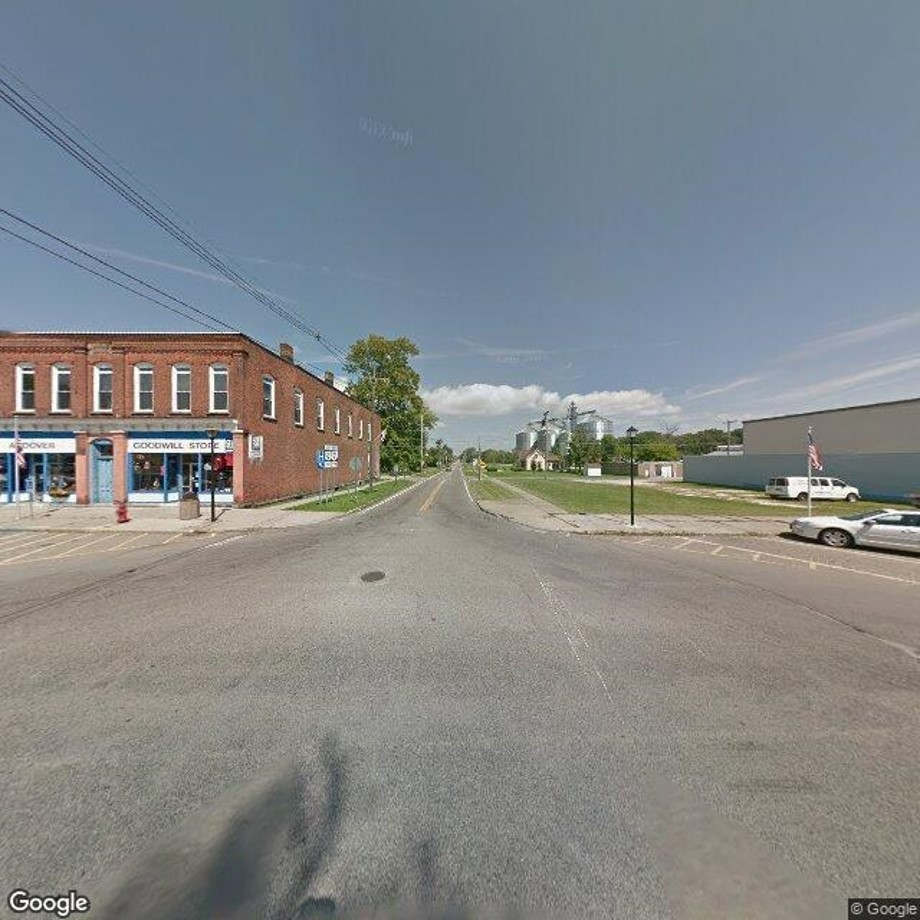
\includegraphics[width=\textwidth]{images/streetview_api_road_before.jpg}
                \caption{Before the election}
                \label{fig:streetview_1}
            \end{subfigure}
            \hfill
            \begin{subfigure}{0.49\textwidth}
                \centering
                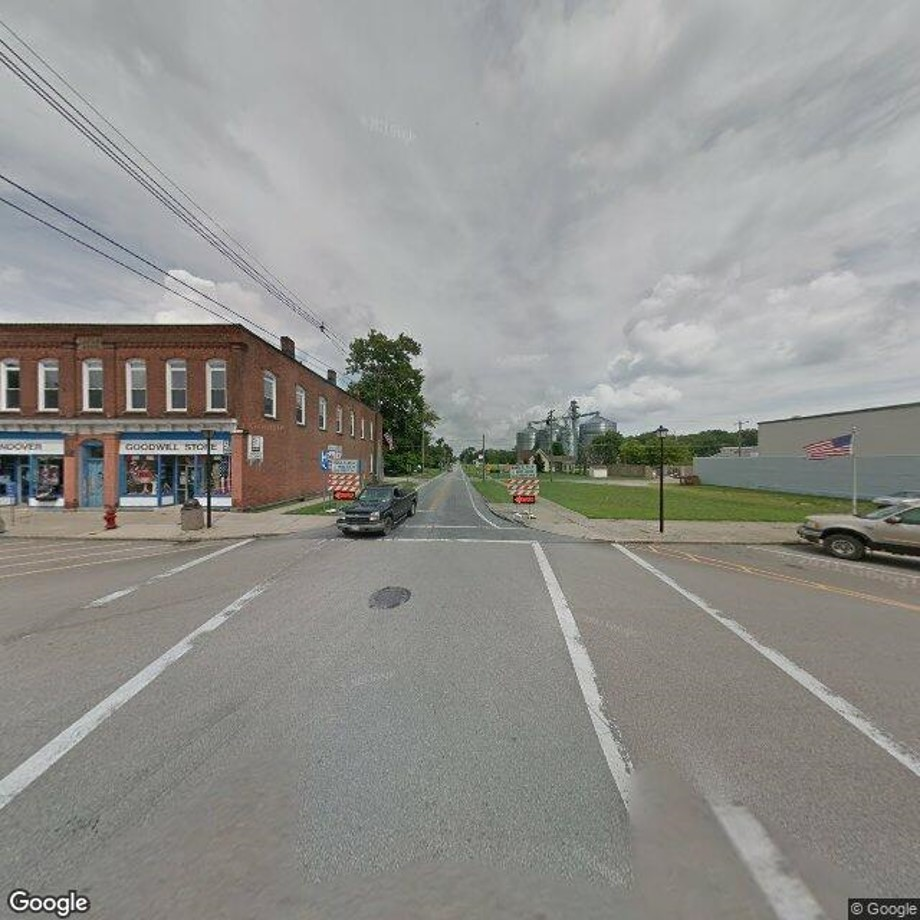
\includegraphics[width=\textwidth]{images/streetview_api_road_after.jpg}
                \caption{After the election}
                \label{fig:streetview_22}
            \end{subfigure}
        \end{figure}
    \end{center}
\end{frame}

%-------------------------------------------------------
% Section 5: Conclusion
%-------------------------------------------------------
\section{Conclusion}

\begin{frame}{Conclusion}
    \begin{itemize}
        \item \textbf{Cutting local road taxes} results in lower road funding and \textbf{long-run declines} in house prices
        \item \textbf{Policy Implication:} Gains from reduced tax bills may be outweighed by \textbf{property value losses}
        \item Local road tax cuts result in a decrease of \$15K (9\%) in house prices over 10 years
        \item Urban areas experience more consistent declines (8\%) than rural areas
        \item Next steps:
            \begin{itemize}
                \item Use audited financial reports of local governments to compute metric 2 for Maintenance spending
                \item Use Streetview images to compute road quality changes i.e. metric 2 for Road Quality
            \end{itemize}
    \end{itemize}
\end{frame}

% Thank you slide
\begin{frame}{Thank You}
    \begin{center}
        % \Large{Thank you for your attention!}\\
        \Large{Questions?}
    \end{center}
\end{frame}

%------------------------------------------------------- 
% Appendix
%-------------------------------------------------------
\appendix
\section{Appendix}


\begin{frame}[label=gdp_and_roads]{Roads and GDP}
    \begin{figure}[ht]
        \centering
        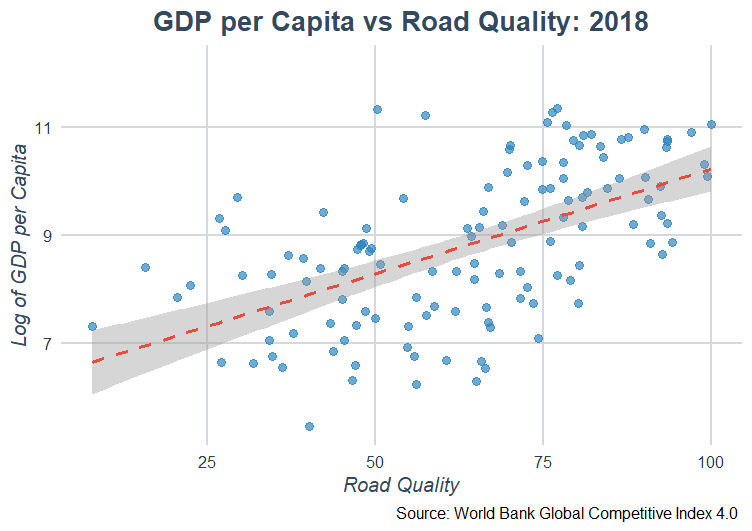
\includegraphics[width=0.8\textwidth]{images/road_quality_vs_gdp_per_cap.png}
        % \caption{Impact of Road Quality on GDP Growth}
        \label{fig:roads_gdp}
    \end{figure}
    \begin{flushright}
        \hyperlink{motivation}{\beamergotobutton{Main}}
    \end{flushright}       
\end{frame}

\begin{frame}[label=odot_who_does_what]{Background}
    Who funds the roads in Ohio?
    \begin{figure}[ht]
        \centering
        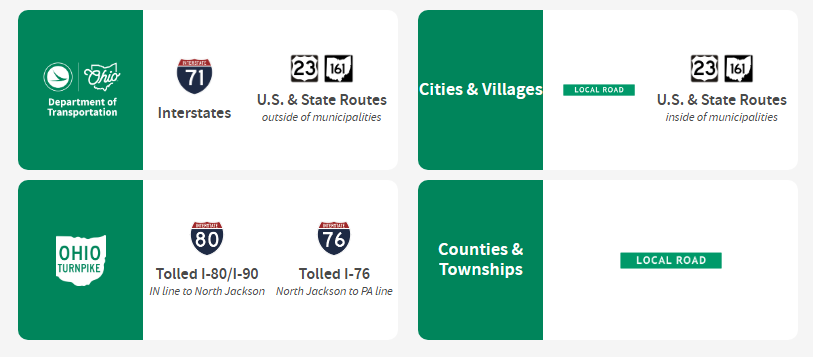
\includegraphics[width=0.9\textwidth]{images/odot_who_does_what.png}
        \caption{Source: Ohio Department of Transportation}
        \label{fig:odot_who_does_what}
    \end{figure}
    \begin{flushright}
        \hyperlink{who_funds_roads}{\beamergotobutton{back to main}}
    \end{flushright}
\end{frame}

\begin{frame}{Background}
    ODOT Disbursement of Funds
    \begin{figure}[ht]
        \centering
        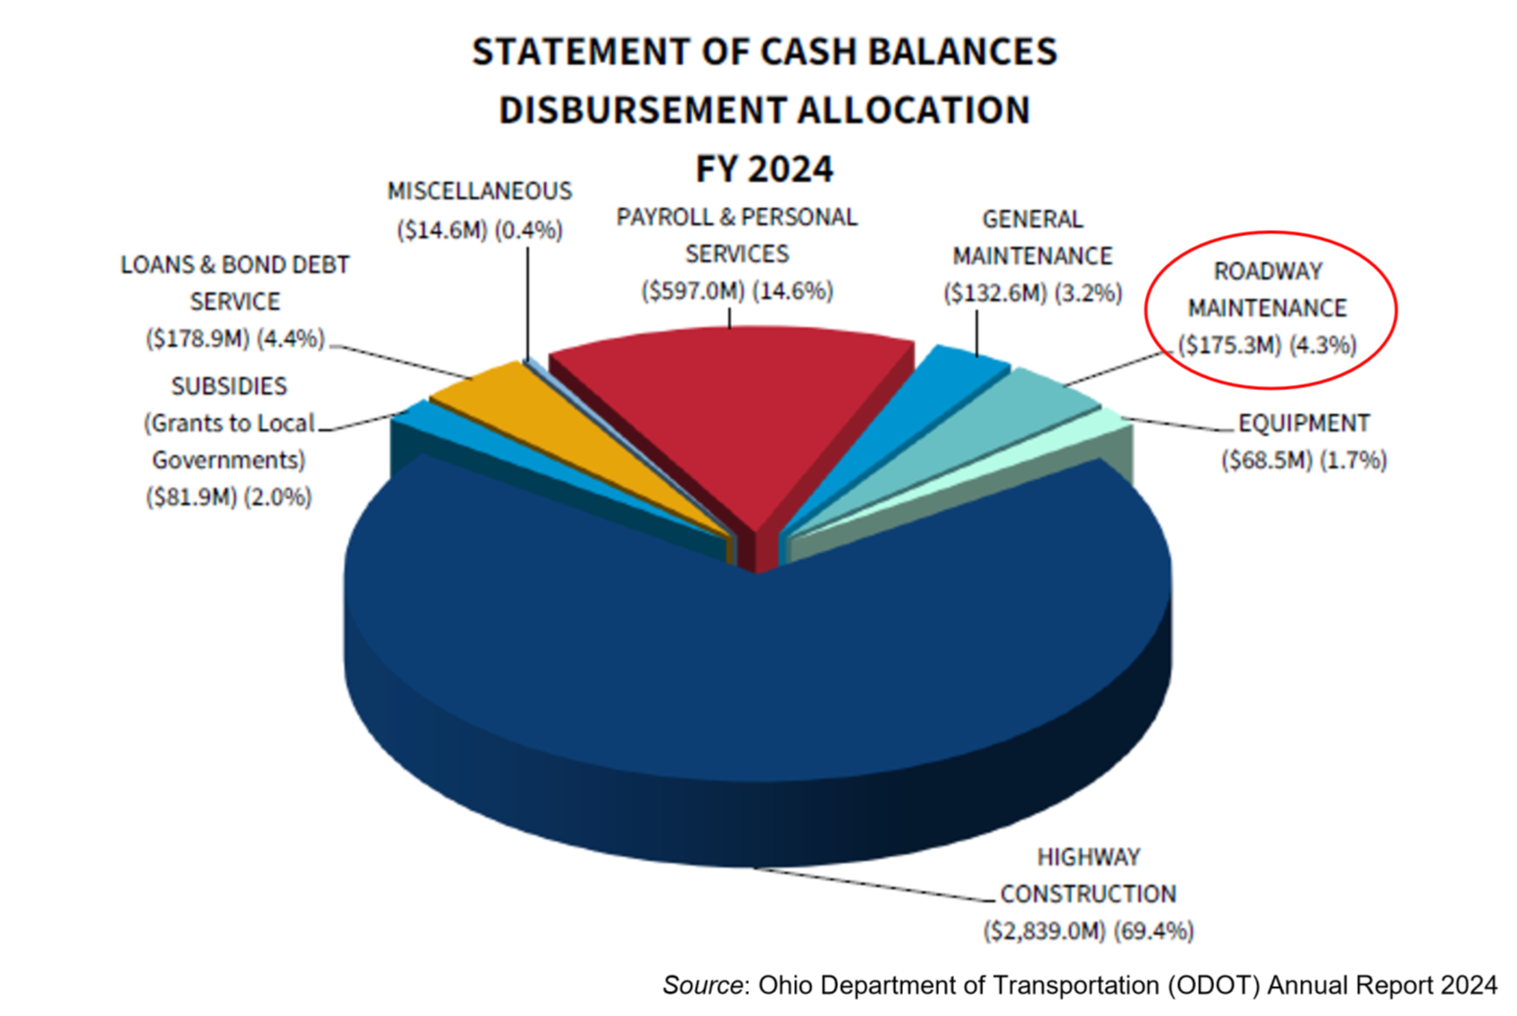
\includegraphics[width=0.9\textwidth]{images/odot_2024.png}
        \caption{Source: Ohio Department of Transportation}
        \label{fig:odot_2024}
    \end{figure}
    \begin{flushright}
        \hyperlink{who_funds_roads}{\beamergotobutton{back to main}}
    \end{flushright}
\end{frame}

% References
% \begin{frame}[allowframebreaks]{References}
%     \bibliographystyle{apalike}
%     \bibliography{aej_references}
% \end{frame}

\begin{frame}{Ohio Auditor of State Reports}
    \begin{figure}[ht]
        \centering
        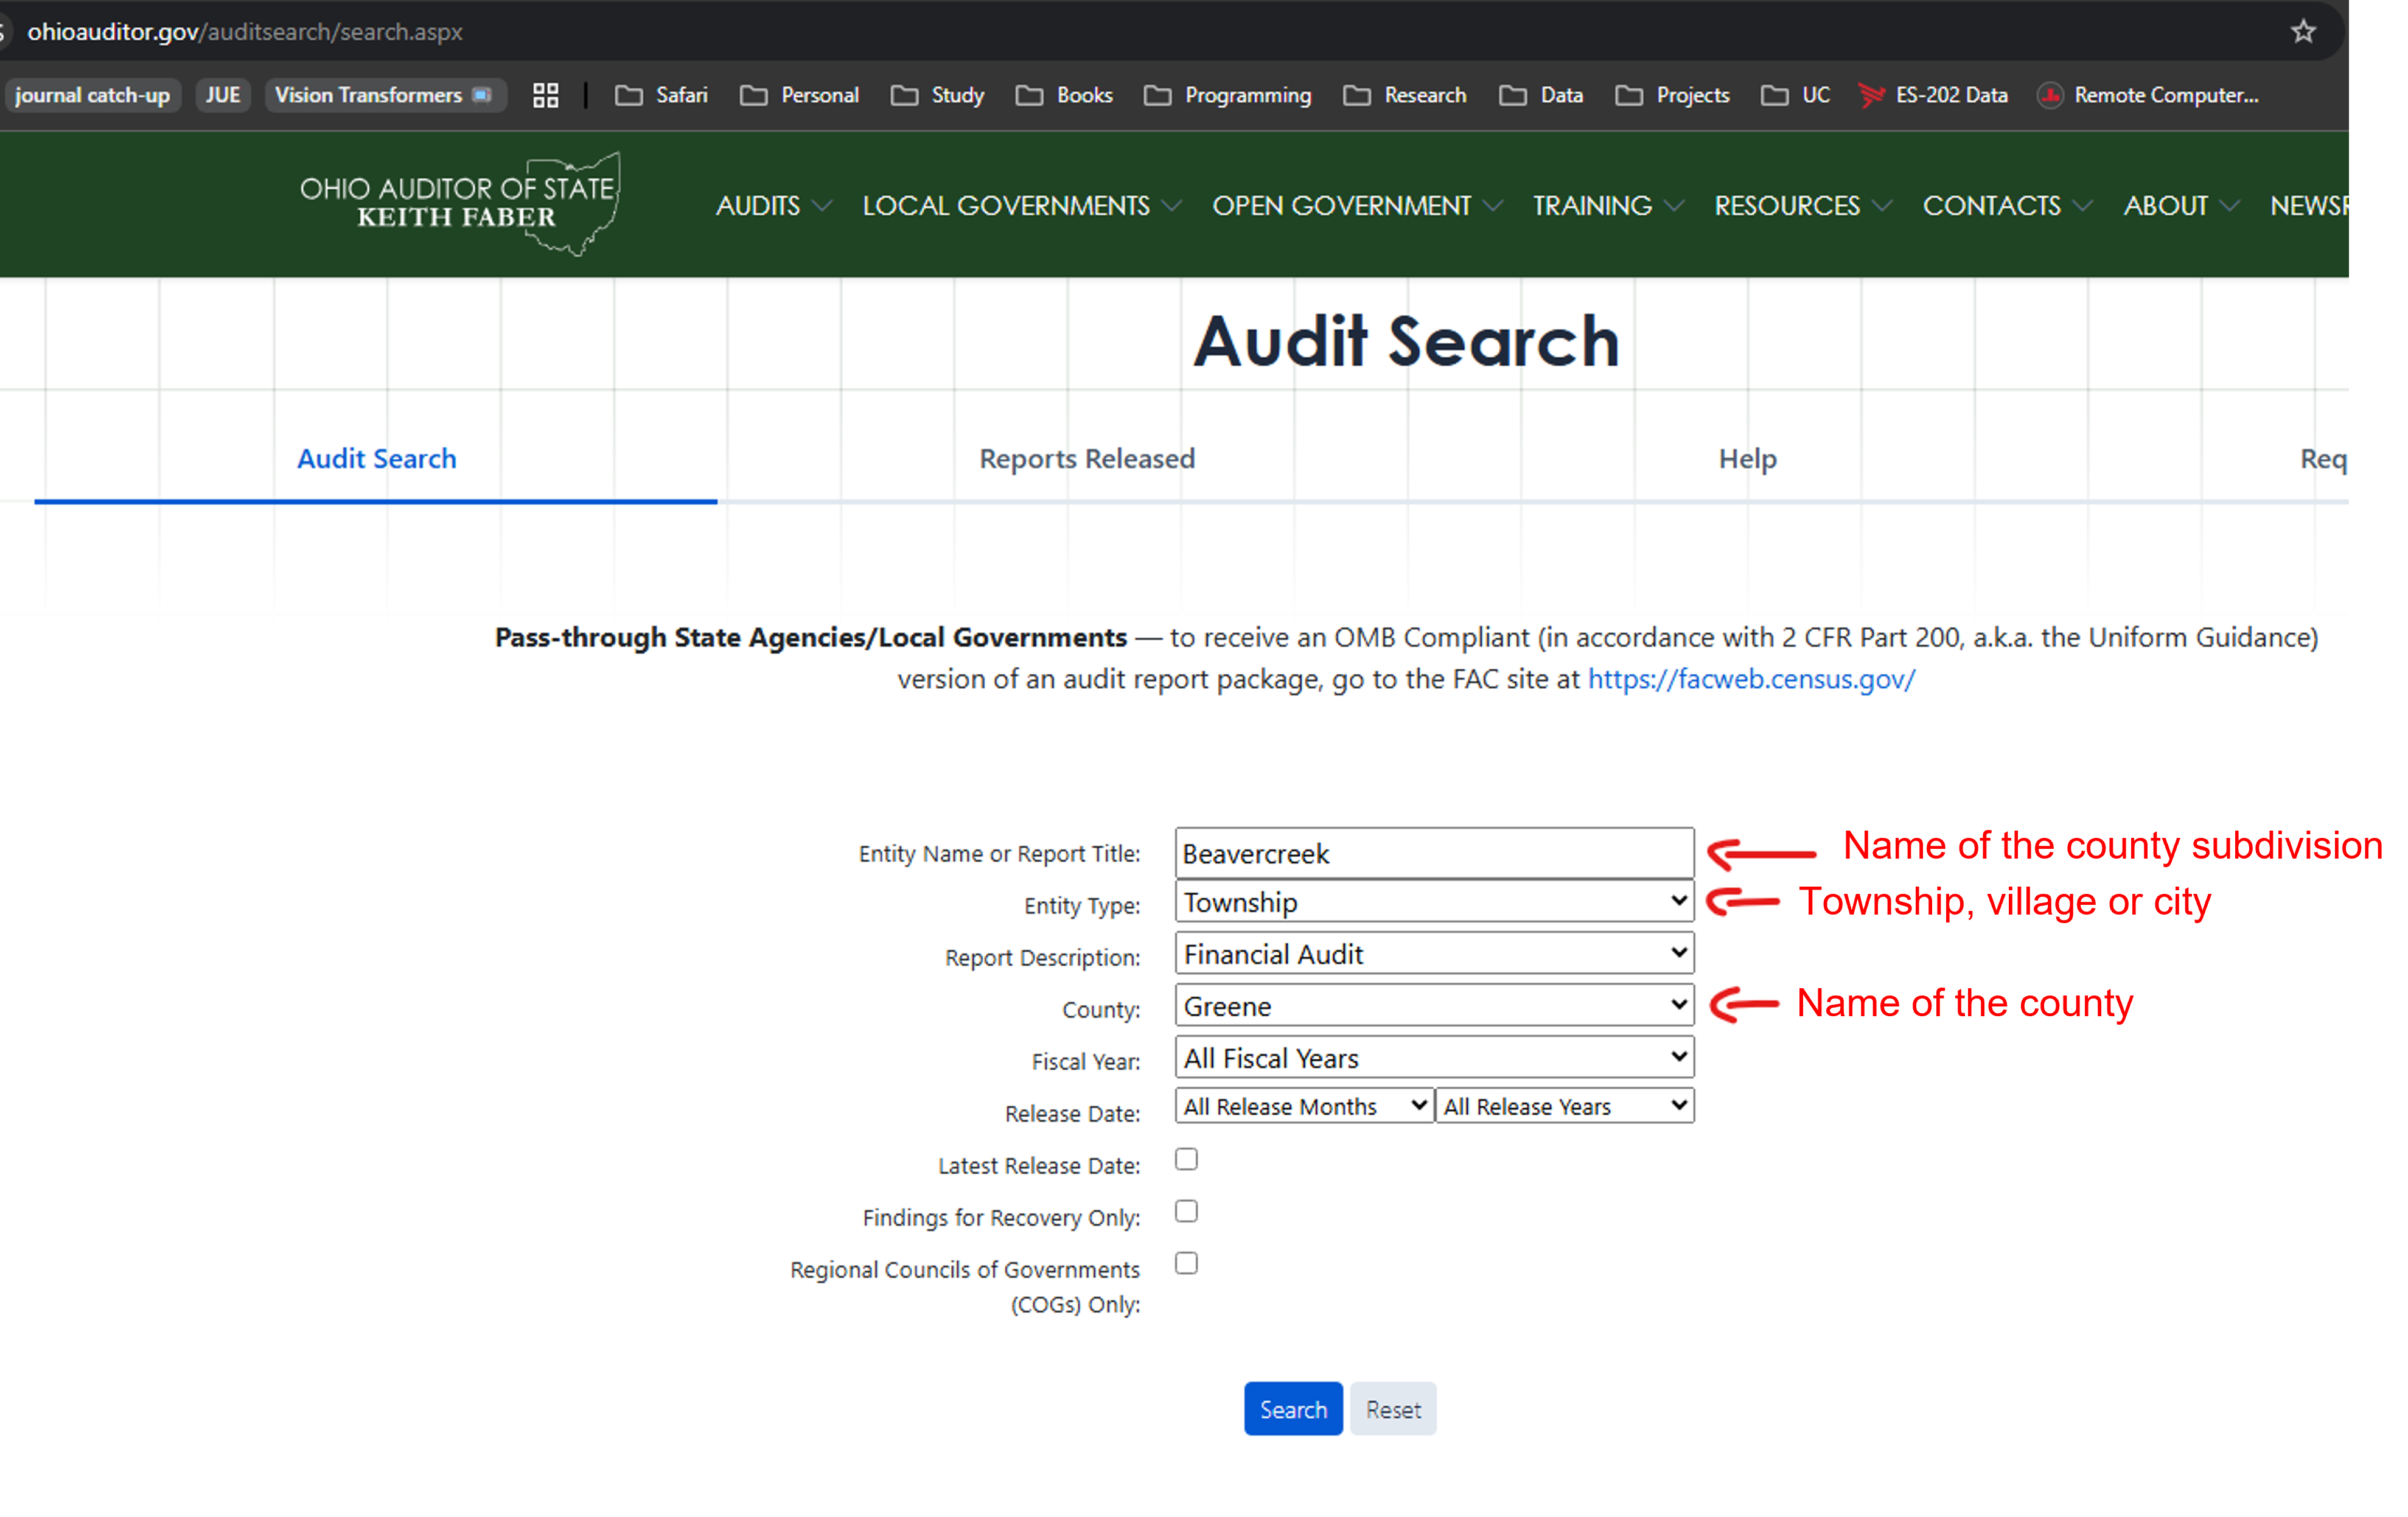
\includegraphics[width=1.0\textwidth]{images/ohio_auditor_of_state_reports_1.png}
        \caption{Ohio Auditor of State Reports Collection}
        \label{fig:auditor_reports1}
    \end{figure}
\end{frame}

\begin{frame}{Ohio Auditor of State Reports}
    \begin{figure}[ht]
        \centering
        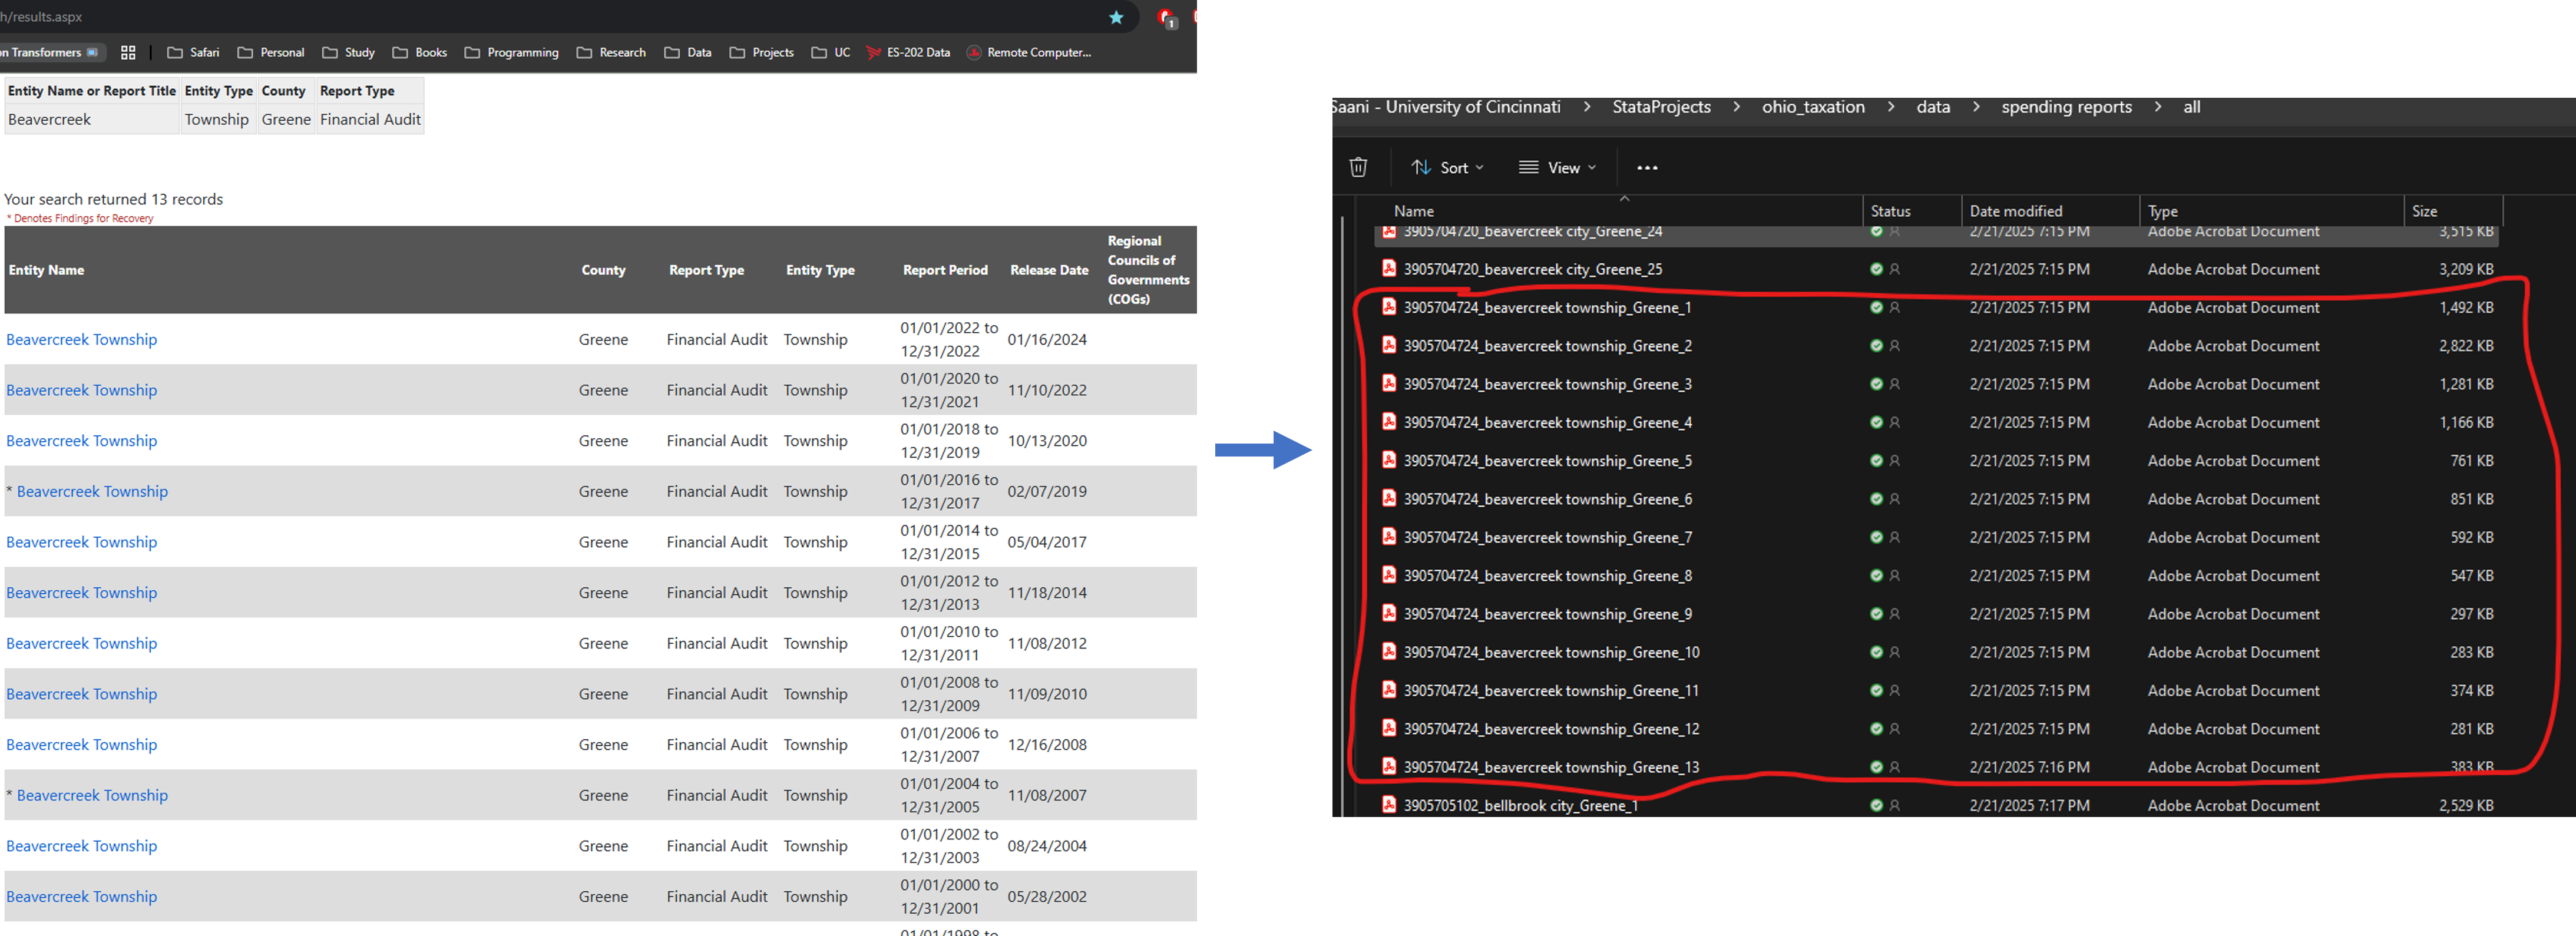
\includegraphics[width=1.0\textwidth]{images/ohio_auditor_of_state_reports_2.png}
        \caption{Ohio Auditor of State Reports Collection}
        \label{fig:auditor_reports2}
    \end{figure}
\end{frame}

\begin{frame}{Covariate Balance Table}
    \begin{figure}[ht]
        \centering
        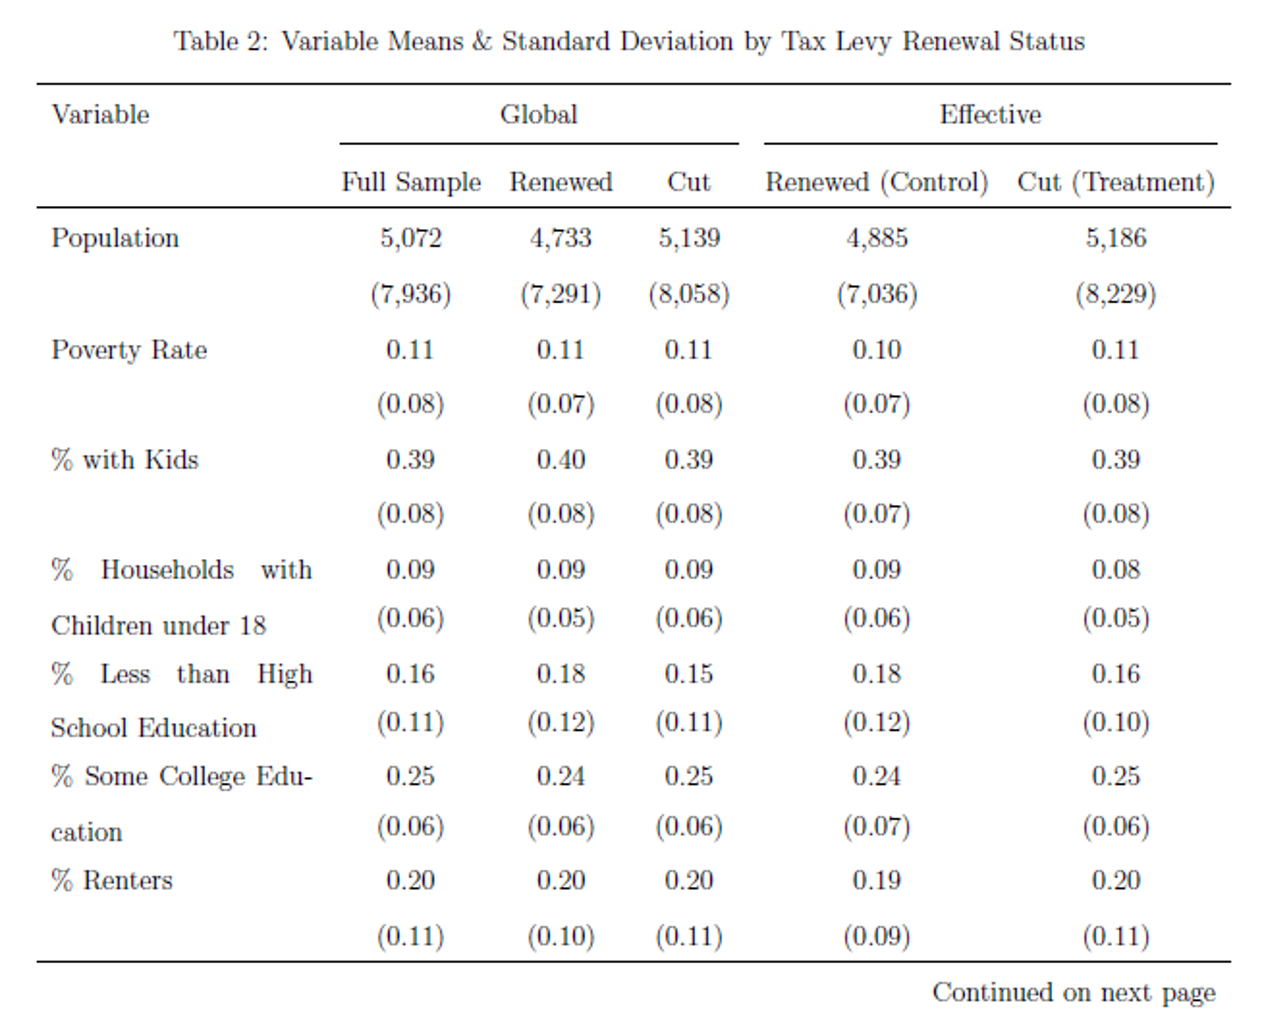
\includegraphics[width=0.9\textwidth]{images/cov_bal_table_1.png}
        \label{fig:covariate_balance_table1}
    \end{figure}
\end{frame}

\begin{frame}{Covariate Balance Table}
    \begin{figure}[ht]
        \centering
        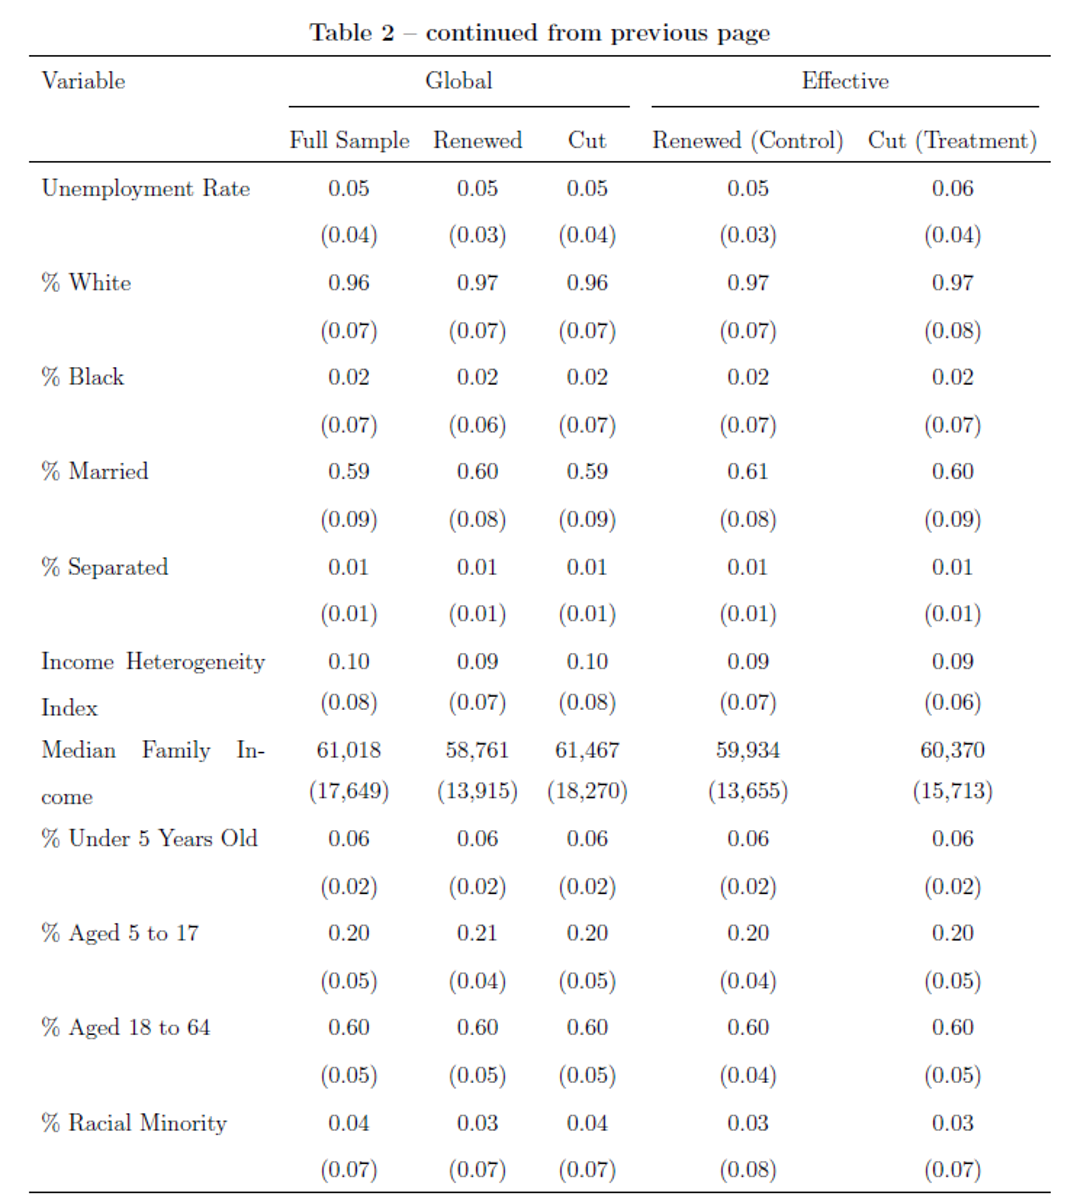
\includegraphics[width=0.65\textwidth]{images/cov_bal_table_2.png}
        \label{fig:covariate_balance_table2}
    \end{figure}
\end{frame}

\begin{frame}{No ``bunching''. Fair elections.}
    \begin{figure}[ht]
        \centering
        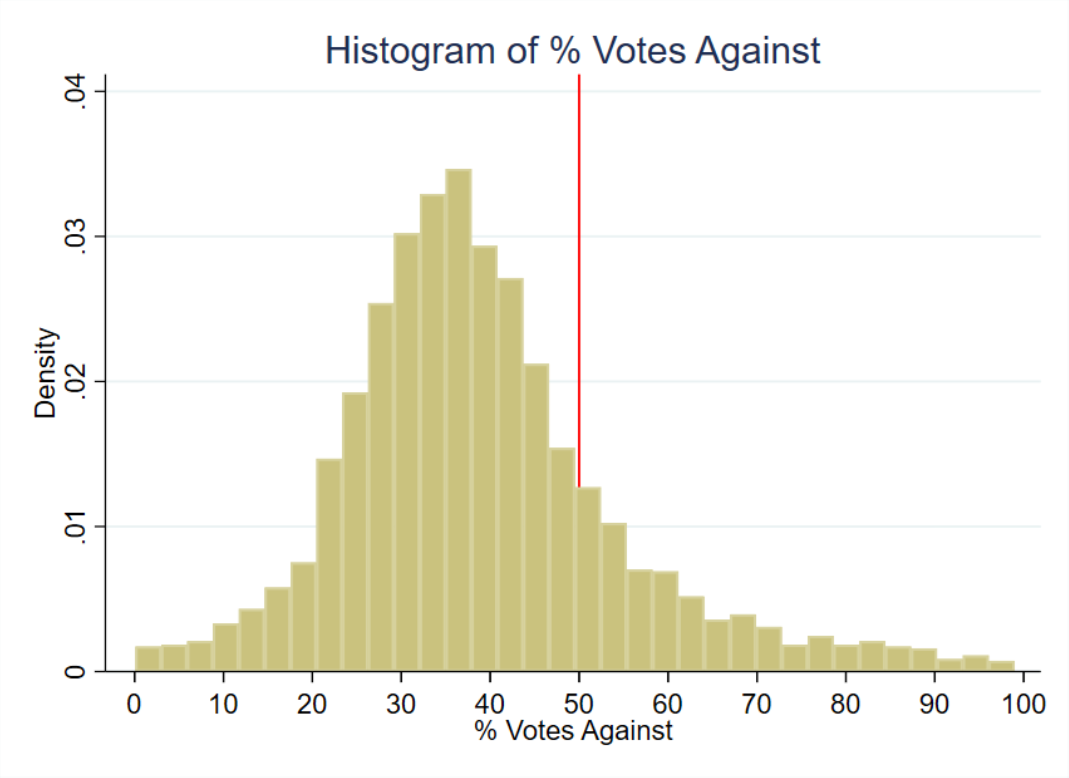
\includegraphics[width=0.8\textwidth]{images/pct_votes_against_histogram.png}
    \end{figure}
\end{frame}

\begin{frame}
    \begin{table}[ht!]
        \centering
        \caption{Correlation of Road Tax Levy Referenda Results with Other Types of Levies}
        \begin{tabular}{lcccccc}
        \toprule
        & Police & Fire & Recreational & School \\
        \midrule
        Estimate & 0.248 & 0.053 & 0.015 & -0.024 \\
        & (0.153) & (0.043) & (0.317) & (0.092) \\
        \bottomrule
        \end{tabular}
        \begin{minipage}{\textwidth}
        \footnotesize
        \textit{Notes:} This table presents coefficients from regressions correlating road tax levy referendum outcomes with outcomes for other types of levies (police, fire, recreational, school). Standard errors are reported in parentheses. All regression control for year and neighborhood fixed effects, as well as neighborhood characteristics. The school levy analysis is conducted at the county level, while all other analyses are at the county subdivisions level. Statistical significance levels are indicated as follows: *** $p<0.01$, ** $p<0.05$, * $p<0.1$.
        \end{minipage}
    \end{table}
\end{frame}

\end{document}

